\documentclass[a4paper,11pt, twoside,openright]{memoir} 	% Openright aabner kapitler paa hoejresider (openany har ikke blanke sider før kapitel) 
%Nanna fjernede fleqn for at centrere ligninger
%til statusseminar fjernes openright
%%%% PACKAGES %%%%

% ¤¤ Oversaettelse og tegnsaetning ¤¤ %
\usepackage[utf8]{inputenc}					% Input-indkodning af tegnsaet (UTF8)
\usepackage[danish]{babel}					% Dokumentets sprog
%\usepackage[english]{babel}					% Dokumentets sprog
\usepackage[T1]{fontenc}					% Output-indkodning af tegnsaet (T1)
\usepackage{ragged2e,anyfontsize}			% Justering af elementer
\usepackage{fixltx2e}						% Retter forskellige fejl i LaTeX-kernen
								
																		
% ¤¤ Figurer og tabeller (floats) ¤¤ %
\usepackage{graphicx} 						% Haandtering af eksterne billeder (JPG, PNG, PDF)
\usepackage{multirow}                		% Fletning af raekker og kolonner (\multicolumn og \multirow)
\usepackage{colortbl} 						% Farver i tabeller (fx \columncolor, \rowcolor og \cellcolor)
\usepackage[dvipsnames]{xcolor}				% Definer farver med \definecolor. Se mere: http://en.wikibooks.org/wiki/LaTeX/Colors
\usepackage{flafter}						% Soerger for at floats ikke optraeder i teksten foer deres reference
\let\newfloat\relax 						% Justering mellem float-pakken og memoir
\usepackage{float}							% Muliggoer eksakt placering af floats, f.eks. \begin{figure}[H]
%\usepackage{eso-pic}						% Tilfoej billedekommandoer paa hver side
%\usepackage{wrapfig}						% Indsaettelse af figurer omsvoebt af tekst. \begin{wrapfigure}{Placering}{Stoerrelse}
%\usepackage{multicol}         	        	% Muliggoer tekst i spalter
%\usepackage{rotating}						% Rotation af tekst med \begin{sideways}...\end{sideways}
\newsubfloat{figure}    

% ¤¤ Matematik mm. ¤¤
\usepackage{amsmath,amssymb,stmaryrd} 		% Avancerede matematik-udvidelser
\usepackage{mathtools}						% Andre matematik- og tegnudvidelser
\usepackage{textcomp}                 		% Symbol-udvidelser (f.eks. promille-tegn med \textperthousand )
\usepackage{siunitx}						% Flot og konsistent praesentation af tal og enheder med \si{enhed} og \SI{tal}{enhed}
\sisetup{output-decimal-marker = {,}}		% Opsaetning af \SI (DE for komma som decimalseparator) 
\usepackage[version=3]{mhchem} 				% Kemi-pakke til flot og let notation af formler, f.eks. \ce{Fe2O3}
%\usepackage{rsphrase}						% Kemi-pakke til RS-saetninger, f.eks. \rsphrase{R1}

% ¤¤ Referencer og kilder ¤¤ %
\usepackage[danish]{varioref}				% Muliggoer bl.a. krydshenvisninger med sidetal (\vref)
\usepackage{natbib}							% Udvidelse med naturvidenskabelige citationsmodeller
%\usepackage{xr}							% Referencer til eksternt dokument med \externaldocument{<NAVN>}
%\usepackage{glossaries}					% Terminologi- eller symbolliste (se mere i Daleifs Latex-bog)


% ¤¤ Misc. ¤¤ %
\usepackage{listings}						% Placer kildekode i dokumentet med \begin{lstlisting}...\end{lstlisting}
\usepackage{lipsum}							% Dummy text \lipsum[..]
\usepackage[shortlabels]{enumitem}			% Muliggoer enkelt konfiguration af lister
\usepackage{pdfpages}						% Goer det muligt at inkludere pdf-dokumenter med kommandoen \includepdf[pages={x-y}]{fil.pdf}	
\pdfoptionpdfminorversion=6					% Muliggoer inkludering af pdf dokumenter, af version 1.6 og hoejere
\usepackage{epstopdf}                       % Muliggoer inklusion af EPS.filer (Encapsulated PostScript), som er vektorbaserede billeder.
\pretolerance=2500 							% Justering af afstand mellem ord (hoejt tal, mindre orddeling og mere luft mellem ord)
% Kommentarer og rettelser med \fxnote. Med 'final' i stedet for 'draft' udloeser hver note en error i den faerdige rapport.
\usepackage[footnote,draft,danish,silent,nomargin]{fixme}		


%%%% CUSTOM SETTINGS %%%%

% ¤¤ Marginer ¤¤ %
\setlrmarginsandblock{3.5cm}{2.5cm}{*}		% \setlrmarginsandblock{Indbinding}{Kant}{Ratio}
\setulmarginsandblock{2.5cm}{3.0cm}{*}		% \setulmarginsandblock{Top}{Bund}{Ratio}
\checkandfixthelayout 						% Oversaetter vaerdier til brug for andre pakker

%	¤¤ Afsnitsformatering ¤¤ %
\setlength{\parindent}{0mm}           		% Stoerrelse af indryk
\setlength{\parskip}{3mm}          			% Afstand mellem afsnit ved brug af double Enter
\linespread{1,1}							% Linie afstand

% ¤¤ Litteraturlisten ¤¤ %
\bibpunct[, ]{[}{]}{,}{a}{,}{,} 				% Definerer de 6 parametre ved Harvard henvisning (bl.a. parantestype og seperatortegn)
\bibliographystyle{bibtex/harvard}			% Udseende af litteraturlisten.



% ¤¤ Indholdsfortegnelse ¤¤ %
\setsecnumdepth{subsection}		 			% Dybden af nummerede overkrifter (part/chapter/section/subsection)
\maxsecnumdepth{subsection}					% Dokumentklassens graense for nummereringsdybde
\settocdepth{subsection} 					% Dybden af indholdsfortegnelsen

% ¤¤ Lister ¤¤ %
\setlist{
  topsep=0pt,								% Vertikal afstand mellem tekst og listen
  itemsep=-1ex,								% Vertikal afstand mellem items
} 

% ¤¤ Visuelle referencer ¤¤ %
\usepackage[colorlinks]{hyperref}			% Danner klikbare referencer (hyperlinks) i dokumentet.
\hypersetup{colorlinks = true,				% Opsaetning af farvede hyperlinks (interne links, citeringer og URL)
    linkcolor = black,
    citecolor = black,
    urlcolor = black
}

% ¤¤ Opsaetning af figur- og tabeltekst ¤¤ %
\captionnamefont{\small\bfseries\itshape}	% Opsaetning af tekstdelen ('Figur' eller 'Tabel')
\captiontitlefont{\small}					% Opsaetning af nummerering
\captiondelim{. }							% Seperator mellem nummerering og figurtekst
\hangcaption								% Venstrejusterer flere-liniers figurtekst under hinanden
\captionwidth{\linewidth}					% Bredden af figurteksten
\setlength{\belowcaptionskip}{0pt}			% Afstand under figurteksten
		
% ¤¤ Opsaetning af listings ¤¤ %
\definecolor{commentGreen}{RGB}{34,139,24}
\definecolor{stringPurple}{RGB}{208,76,239}

\lstset{language=Matlab,					% Sprog
	basicstyle=\ttfamily\scriptsize,		% Opsaetning af teksten
	keywords={for,if,while,else,elseif,		% Noegleord at fremhaeve
			  end,break,return,case,
			  switch,function},
	keywordstyle=\color{blue},				% Opsaetning af noegleord
	commentstyle=\color{commentGreen},		% Opsaetning af kommentarer
	stringstyle=\color{stringPurple},		% Opsaetning af strenge
	showstringspaces=false,					% Mellemrum i strenge enten vist eller blanke
	numbers=left, numberstyle=\tiny,		% Linjenumre
	extendedchars=true, 					% Tillader specielle karakterer
	columns=flexible,						% Kolonnejustering
	breaklines, breakatwhitespace=true,		% Bryd lange linjer
}

% ¤¤ Navngivning ¤¤ %   
%% I denne engelsk udgave, er det kun de fremhævede der skal bruges. De er ændret til engelsk stavemåde%%
%\addto\captionsdanish{
	\renewcommand\appendixname{Appendix}
%	\renewcommand\contentsname{Indholdsfortegnelse}	
	\renewcommand\appendixpagename{Appendix}
	\renewcommand\appendixtocname{Appendix}
	\renewcommand\cftchaptername{\chaptername~}				% Skriver "Kapitel" foran kapitlerne i indholdsfortegnelsen
	\renewcommand\cftappendixname{\appendixname~}			% Skriver "Appendiks" foran appendiks i indholdsfortegnelsen
%}




% ¤¤ Kapiteludssende ¤¤ %
\definecolor{numbercolor}{gray}{0.5}		% Definerer en farve til brug til kapiteludseende
\newif\ifchapternonum

\makechapterstyle{jenor}{					% Definerer kapiteludseende frem til ...
  \renewcommand\beforechapskip{0pt}
  \renewcommand\printchaptername{}
  \renewcommand\printchapternum{}
  \renewcommand\printchapternonum{\chapternonumtrue}
  \renewcommand\chaptitlefont{\fontfamily{pbk}\fontseries{db}\fontshape{n}\fontsize{25}{35}\selectfont\raggedleft}
  \renewcommand\chapnumfont{\fontfamily{pbk}\fontseries{m}\fontshape{n}\fontsize{1in}{0in}\selectfont\color{numbercolor}}
  \renewcommand\printchaptertitle[1]{%
    \noindent
    \ifchapternonum
    \begin{tabularx}{\textwidth}{X}
    {\let\\\newline\chaptitlefont ##1\par} 
    \end{tabularx}
    \par\vskip-2.5mm\hrule
    \else
    \begin{tabularx}{\textwidth}{Xl}
    {\parbox[b]{\linewidth}{\chaptitlefont ##1}} & \raisebox{-15pt}{\chapnumfont \thechapter}
    \end{tabularx}
    \par\vskip2mm\hrule
    \fi
  }
}											% ... her

\makechapterstyle{ST4}{					% Definerer kapiteludseende frem til ...
	\renewcommand\beforechapskip{0pt}
	\renewcommand\printchaptername{}
	\renewcommand\printchapternum{}
	\renewcommand\printchapternonum{\chapternonumtrue}
	\renewcommand\chaptitlefont{\fontfamily{put}\fontseries{m}\fontshape{n}\fontsize{30}{30}\selectfont\raggedright}
	\renewcommand\chapnumfont{\fontfamily{put}\fontseries{m}\fontshape{n}\fontsize{1in}{0in}\selectfont\color{numbercolor}}
	\renewcommand\printchaptertitle[1]{%
		\noindent
		\ifchapternonum
		\begin{tabularx}{\textwidth}{X}
			{\raisebox{-10mm}{\let\\\newline\chaptitlefont ##1\par} }
		\end{tabularx}
		\par\vskip2mm\hrule\vskip-7mm
		\else
		\begin{tabularx}{\textwidth}{Xl}
			{\parbox[b]{\linewidth}{\chaptitlefont ##1}} & {\chapnumfont \thechapter}
		\end{tabularx}
		\par\vskip2mm\hrule\vskip-7mm
		\fi
	}
}											% ... her

\chapterstyle{ST4}						% Valg af kapiteludseende - Google 'memoir chapter styles' for alternativer




%\chapterstyle{jenor}						% Valg af kapiteludseende - Google 'memoir chapter styles' for alternativer

% ¤¤ Sidehoved ¤¤ %

\makepagestyle{Uni}							% Definerer sidehoved og sidefod udseende frem til ...
\makepsmarks{Uni}{%
	\createmark{chapter}{left}{shownumber}{}{. \ }
	\createmark{section}{right}{shownumber}{}{. \ }
	\createplainmark{toc}{both}{\contentsname}
	\createplainmark{lof}{both}{\listfigurename}
	\createplainmark{lot}{both}{\listtablename}
	\createplainmark{bib}{both}{\bibname}
	\createplainmark{index}{both}{\indexname}
	\createplainmark{glossary}{both}{\glossaryname}
}
\nouppercaseheads											% Ingen Caps oenskes

\makeevenhead{Uni}{Gruppe 17gr5403}{}{\leftmark}				% Definerer lige siders sidehoved (\makeevenhead{Navn}{Venstre}{Center}{Hoejre})
\makeoddhead{Uni}{\rightmark}{}{Aalborg Universitet}			% Definerer ulige siders sidehoved (\makeoddhead{Navn}{Venstre}{Center}{Hoejre})
\makeevenfoot{Uni}{\thepage}{}{}							% Definerer lige siders sidefod (\makeevenfoot{Navn}{Venstre}{Center}{Hoejre})
\makeoddfoot{Uni}{}{}{\thepage}								% Definerer ulige siders sidefod (\makeoddfoot{Navn}{Venstre}{Center}{Hoejre})
\makeheadrule{Uni}{\textwidth}{0.5pt}						% Tilfoejer en streg under sidehovedets indhold
\makefootrule{Uni}{\textwidth}{0.5pt}{1mm}					% Tilfoejer en streg under sidefodens indhold

\copypagestyle{Unichap}{Uni}								% Sidehoved for kapitelsider defineres som standardsider, men med blank sidehoved
\makeoddhead{Unichap}{}{}{}
\makeevenhead{Unichap}{}{}{}
\makeheadrule{Unichap}{\textwidth}{0pt}
\aliaspagestyle{chapter}{Unichap}							% Den ny style vaelges til at gaelde for chapters
															% ... her
															
\pagestyle{Uni}												% Valg af sidehoved og sidefod (benyt "plain" for ingen sidehoved/fod)


%%%% CUSTOM COMMANDS %%%%

% ¤¤ Billede hack ¤¤ %										% Indsaet figurer nemt med \figur{Stoerrelse}{Fil}{Figurtekst}{Label}
\newcommand{\figur}[4]{
		\begin{figure}[H] \centering
			\includegraphics[width=#1\textwidth]{billeder/#2}
			\caption{#3}\label{#4}
		\end{figure} 
}

% ¤¤ Specielle tegn ¤¤ %
\newcommand{\decC}{^{\circ}\text{C}}
\newcommand{\dec}{^{\circ}}
\newcommand{\m}{\cdot}
\DeclareMathSymbol{*}{\mathbin}{symbols}{"01}    % Lav * om til \cdot

%% Til tabeller
\usepackage{makecell}
\usepackage{longtable}


\usepackage{xcolor}
\usepackage{ragged2e}
\usepackage{paracol}
\usepackage{blindtext}

\usepackage{supertabular}

\usepackage{lscape}
\usepackage{csquotes}
%\usepackage[switch, modulo]{lineno}
\usepackage{lineno}
%\usepackage{arydshln}
\usepackage{tabu}
\usepackage{booktabs}

%Acronym liste%
\usepackage[nopostdot, style=super, nogroupskip]{glossaries}   %nopostdot: fjerner punktum, style=super: Ordene starter fra samme punkt
\setacronymstyle{long-short}
\renewcommand{\glsnamefont}[1]{\textbf{#1}}                     %For at gøre forkortelser fed i listen


%\input{formalia/forkortelser}
\makenoidxglossaries
\glsenableentrycount


%%%% ORDDELING %%%%

%\hyphenation{}

%%Farver
\definecolor{table}{gray}{0.9}
\definecolor{lightred}{cmyk}{0,0.49,54}
%\usepackage{lastpage}
											% Preamble indlaeses
\raggedbottom													% Soerger for at LaTeX ikke "straekker" teksten

%\includeonly{file1,file2}										% Inkluder kun specifikke filer (kommasepareret liste)

\begin{document}												% Starter dokumentet - obligatorisk


\frontmatter													% Forindhold - nummereres med romertal

\thispagestyle{empty}
\newcommand{\HRule}{\rule{\linewidth}{0.5mm}} % Defines a new command for the horizontal lines, change thickness here

\begin{center} % Center everything on the page
 %----------------------------------------------------------------------------------------
%	HEADING SECTIONS
%----------------------------------------------------------------------------------------

\textsc{\LARGE Aalborg Universitet}\\[1.0cm] % Name of your university/college
\textsc{\Large Sundhedsteknologi}\\[0.5cm] % Major heading such as course name
\textsc{\Large Bachelor Projekt}\\[0.5cm] % Major heading such as course name
\textsc{\large Gruppe 18gr6405}\\[0.5cm] % Minor heading such as course title

%----------------------------------------------------------------------------------------
%	TITLE SECTION
%----------------------------------------------------------------------------------------

\HRule \\[0.4cm]
{ \huge \bfseries Udvikling af brugervenlig app til hjemmemonitorering}\\[0.2cm] % Title of your document
\HRule \\[0.4cm]
%----------------------------------------------------------------------------------------
%	AUTHOR SECTION
%----------------------------------------------------------------------------------------

\emph{Forfattere:}\\
{\large Lissi Thi Kim Phuong Nguyen \\ Mads Fedders \\ Munira Farah \\ Nicholas L. Jessen \\ Sarah Søltoft Rasmussen \\[1.0cm] % Editor list

\emph{Hovedvejleder:}\\
{\large Jacob Melgaard \par}\\[0.5cm] % Supervisor list

\emph{Bivejleder:}\\
{\large Kasper Sørensen  \par}\\[2.0cm] % Supervisor list

%----------------------------------------------------------------------------------------
%	DATE SECTION
%----------------------------------------------------------------------------------------

%{\large \ 24$^{th}$ May 2017}\\[0.5cm] % Date, change the \today to a set date if you want to be precise

%----------------------------------------------------------------------------------------
%	LOGO SECTION
%----------------------------------------------------------------------------------------


\includegraphics[height=4cm]{Billeder/AAU-logo-stud-DK-RGB} % Include a department/university logo - this will require the graphicx package
 
%----------------------------------------------------------------------------------------

\vfill % Fill the rest of the page with whitespace
\end{center}
\cleardoublepage												% Indsaetter tom side, saa naeste kapitel starter paa hoejre side (hvis noedvendigt)
% Dette er LaTeX-versionen af titelbladet for TNB studenterrapporter
% Filen kræver:
% Universitetets logo:  AAU-logo-stud-UK eller AAU-logo-stud-DK
% Synopsis: En fil ved navn synopsis.tex

% Udarbejdet af: Jesper Nørgaard (jesper@noergaard.eu) 10. april 2012

\phantomsection
\pdfbookmark[0]{Titelblad}{titelblad}
\thispagestyle{empty}

\begin{minipage}[t]{0.48\textwidth}
\vspace*{-25pt}			%\vspace*{-9pt}

\includegraphics[height=4cm]{Billeder/AAU-logo-stud-UK-RGB}
\end{minipage}
\hfill
\begin{minipage}[t]{0.48\textwidth}
{\small 
\textbf{School of Medicine and Health}  \\
Sundhedsteknologi \\
Fredrik Bajersvej 7A \\
9000 Aalborg \\
http://www.smh.aau.dk}
\end{minipage}

\vspace*{1cm}

\begin{minipage}[t]{0.48\textwidth}
\textbf{Titel:} %\\[5pt]\bigskip\hspace{2ex}
\\\hspace*{2ex} 
Udvikling af brugervenlig app\\\hspace*{2ex} 
til hjemmemonitorering  \\\hspace*{2ex} 

\textbf{Projekt:} %\\[5pt]\bigskip\hspace{2ex}
\\\hspace*{2ex}
Bachelor Projekt \\\hspace*{2ex}

\textbf{Projektperiode:} %\\[5pt]\bigskip\hspace{2ex}
\\\hspace*{2ex}
Februar 2018 - Maj 2018 \\\hspace*{2ex}

\textbf{Projektgruppe:} %\\[5pt]\bigskip\hspace{2ex}
\\\hspace*{2ex}
18gr6405 \\\hspace*{2ex}

\textbf{Gruppemedlemmer:} %\\[5pt]\hspace*{2ex}
\\\hspace*{2ex}
Lissi T. K. P. Nguyen\\\hspace*{2ex}
Mads Fedders \\\hspace*{2ex}
Munira Farah\\\hspace*{2ex}
Nicholas L. Jessen\\ \bigskip\hspace{2ex}
Sarah Søltoft Rasmussen\\\hspace*{2ex}


\textbf{Hovedvejleder:} %\\[5pt]\hspace*{2ex}
\\\hspace*{2ex}Jacob Melgaard
 \\ \bigskip\hspace{2ex}
 
 
\textbf{Bivejleder:} %\\[5pt]\hspace*{2ex}
\\\hspace*{2ex}Kasper Sørensen
%\\\hspace*{2ex}
 \\ \bigskip\hspace{2ex}

\vspace*{0.5cm}

\textbf{Sider:}  XX\\
\textbf{Appendiks:} XX \\ 
\textbf{Afsluttet:} 28-05-2018

\end{minipage}
\hfill
\begin{minipage}[t]{1.5\textwidth}%483
Synopsis: \\[1pt]
\fbox{\parbox{8.5cm}{Her skriver vi vores synopsis}}
\end{minipage}

\vfill

{\footnotesize\itshape Rapportens indhold er frit tilgængeligt, men offentliggørelse (med kildeangivelse) må kun ske efter aftale
med forfatterne.}

% Rapportens indhold er frit tilgængeligt, men offentliggørelse (med kildeangivelse) må kun ske efter aftale med forfatterne.
% The content of the report is freely available, but publication (with source reference) may only take place in agreement with the authors.
                                   %Her indsættes titelblad
\cleardoublepage
\chapter*{Forord}
Her skriver vi vores forord...


\phantom{Luft}
\phantom{Luft}
\phantom{Luft}
\phantom{Luft}
\phantom{Luft}
\phantom{Luft}

\begin{table}[H]
	\centering
		\begin{tabular}{c c c}
		&&\\
			\underline{\phantom{mmmmmmmmmmmmmm}} & \underline{\phantom{mmmmmmmmmmmmmm}} & \underline{\phantom{mmmmmmmmmmmmmm}} \\ \\
			Lissi T. K. P. Nguyen			& Mads Fedders 		& Munira Farah 			\\
			&&\\
			&&\\
			&&\\
			&&\\
			
		 																				
																					
		\end{tabular}
		\begin{tabular}{c c}
		    &  \\
		     \underline{\phantom{mmmmmmmmmmmmmm}} & \underline{\phantom{mmmmmmmmmmmmmm}} & \\
			Nicholas L. Jessen			& Sarah Søltoft	Rasmussen		\\
			&&\\
			&&\\
		    & 
		\end{tabular}
\end{table}

\newpage


\section*{Læsevejledning} 
Her skriver vi vores læsevejledning                                      %Her indsættes forord
\cleardoublepage
\printnoidxglossary[sort=word, title=Akronymer, nonumberlist=true]  
\cleardoublepage

%%%% Indholdsfortegnelse (TOC) %%%%

%\phantomsection											    % Kunstigt afsnit, som hyperlinks kan 'holde fast i'
%\pdfbookmark[0]{Indholdsfortegnelse}{indhold}					% Tildeler en klikbar bookmark til den endelige PDF
\tableofcontents*												%  Indholdsfortegnelsen (kaldet ToC) 

%\addtocontents{toc}{\protect\newpage}							% Fremtvinger sideskift i ToC hvis noedvendig (der hvor koden placeres)


\mainmatter														% Hovedindhold - nummereres fra side 1

%%%% Rapportindhold %%%% 										% Rapportindholdet boer IKKE indeholde broedtekst - KUN includede filer!

%%Statusseminar%%
%\include{Statusseminar/Statusseminar}

%% Indledning %%


%% Problemanalyse %%
\chapter{Problemanalyse}
\textit{Dette kapitel har til formål at skabe en grundlæggende forståelse for patientgruppens sygdom, diversitet, forløb og efterforløb. Herudover er der undersøgt hvorledes telemonitorering kan bidrage til et bedre efterforløb for patientgruppen, samt de mulige it-løsninger hertil.}

\section{Hjertesvigt} \label{hjertesvigt}

%De patofysiologiske processer er yderst komplekst. Flere forskellige hypoteser som forklarer tilstanden er fremsat. \citep{Abraham2007}Hjertesvigt forbliver ufuldstændigt forstået af forskere, og der er ikke en enkelt samlet ramme, som har vist sig holdbar \citep{Coronel2001}. 
Hjertesvigt er en progressiv lidelse, som forekommer sekundært til abnormaliteter i hjertemusklens struktur, funktion eller begge. Abnormaliteteten, uanset årsagen, resulterer i at hjertet har en manglende evne til at imødekomme kroppens metaboliske behov \citep{Shah2011}\citep{Fletcher2001}\citep{Francis1998}\citep{Mudd2008}. Dette syndrom er associeret med nedsat motionstolerance, dyspnø under hvile og anstrengelse og ødemer i underekstremitet \citep{Francis1998}. Derudover ses fund som øget halsvenetryk, krepetitioner i lungerne og perifere ødemer \citep{heartfailure}.\\
Hjertesvigt er et almindeligt klinisk syndrom, men de patofysiologiske faktorer kan variere betydeligt mellem patienterne \citep{Parmley1985}. Selvom der er mange årsager eller tilstande som kan føre til hjertesvigt, så er de mest almindelige årsager ukontrolleret hypertension, koronararteriesygdom og mitral eller aortaklap dysfunktion \citep{Fletcher2001}. Derudover ses der også sygdomme som kronisk øger belastningen på hjertet, som ved tab af myocytter pga. hjerteinfarkt \citep{Shah2011}. \\
Et normalt fungerende hjerte er i stand til at foretage præcise justeringer i slagvolumen til at imødekomme ændringer i kroppens metaboliske behov ved hvile og motion. Disse fysiologiske variationer i slagvolumen er mulige grundet hjertets elasticitet og er sammen med minutvolumen påvirket af fire variable: inotropi eller hjertets kontraktilitet, preload eller diastolisk fyldningsvolume, afterload eller mængden af tryk som ventriklen skal overkomme for at aortaklappen åbnes, og kronotropi eller hjerterytme \citep{Fletcher2001}.  \\
Overordnet findes to typer af hjertesvigt: systolisk og diastolisk. Forskellen mellem systolisk og diastolisk dysfunktion kan bestemmes vha. ejection fraction (EF). Systolisk dysfunktion er karakteriseret ved EF mindre end 40 \% \citep{Consensus1999} \citep{Fletcher2001}. Systolisk dysfunktion er karakteriseret ved en reduceret venstre ventrikel kontraktilitet, der ofte resulterer i et dilateret hjerte, som ikke er i stand til at vedligeholde en tilstrækkelig minutvolumen \citep{Mudd2008} \citep{Consensus1999} \citep{Fletcher2001}. Hos patienter med diastolisk hjertesvigt, er volumen i den venstre ventrikel typisk normal, hvor EF er større end 50 \% \citep{Ruzumna1996},  og oftest ses hypertrofisk kardiomyopati \citep{Braunwald2013}. Hjertet er i dette tilfælde ikke i stand til at fylde sig tilstrækkeligt under diastole, hvilket fører til en nedsat slagvolumen, nedsat minutvolumen og symptomer på hjertesvigt \citep{Ruzumna1996} \citep{Willerson1995}\citep{Fletcher2001}. Generelt er det iskæmiske hjertesygdomme, som er den mest almindelige årsag til systolisk dysfunktion, mens venstre ventrikel hypertrofi, sekundært til hypertension eller klap abnormaliteter, udgør størstedelen ved diastolisk dysfunktion \citep{Mcalister1997}.\\
Når der er en nedsat minutvolumen og deraf nedsat gennemsnitligt arterietryk, er der en stimulering af flere neurohormonelle systemer som vedligeholder hæmodynamisk stabilitet \citep{Mccance1998}. Her kan kan blandt andet nævnes en stimulering af det sympatiske nervesysstem (SNS) til at udskille adrenalin og noradrenalin, som medfører en øget perifer vaskulær modstand, hjerterytme og kontraktilitet \citep{Fletcher2001}. Redistribuering af blodflow, som resultat af SNS stimulering, nedsætter renal perfusion, som medfører en aktivering af renin-angiotensin-aldosteron-systemet (RAAS). Dette vil efterfølgende medføre vasokonstriktion og retention af vand og salt \citep{Mccance1998}. Renal retention af salt og vand sammen med en øget perifer vaskulær modstand fører til en øget preload og afterload, som medvirker til pulmonale og vaskulære ødemer og skaber symptomer som er karakteristisk ved hjertesvigt \citep{Mccance1998}.\\
En aktiverering af SNS og RAAS vil på længere sigt medføre remodellering af ventriklerne og yderligere myokardieskader, hvorved en ond cirkel opstår \citep{Braunwald2013}. Ventrikulær remodellering er en kompleks patofysiologisk proces som manifesterer sig som ændringer i størrelse, form og funktion af hjertet. Eksempelvis vil en skade på hjertet medføre myocytnekrose \citep{Cohn2000}. Dette ses blandt andet hos patienter med koronararteriesygdom, som har haft en eller flere myokardieinfarkter \citep{Page1971}. Som et forsøg på at vedligholde minutvolumen efter tab af kontraktilt væv, vil de overlevende myocytter forlænge og hypertrofere. Som ventriklerne forstørres vil ventiklernes vægge blive tyndere og begynde at dilatere, hvilket resulterer i dilateret kardiomyopati \citep{Cohn2000}. Remodellering kan forekomme efter akut hjerteinfarkt eller globalt som resultat af kardiomyopati. Hvis det ikke behandles, kan ændringen i venstre ventrikels geometri resultere i ændringer i muskelfunktionen og kan føre til udvikling af sekundær mitral insufficiens, som efterfølgende fører til yderligere forringelse af minutvolumen \citep{Gheorghiade1998}.\\
Initielt er disse kompensatoriske mekanismer gavnlige, men over tid vil disse dog stresse hjertet yderligere og forværre hjertesvigt \citep{Mccance1998} som i sidste ende øger sandsynligheden for organsvigt eller en forværring i den klinisk prognose\citep{Mudd2008}. Her kan hjerterytmen nævnes, der som regel er øget ved hjertesvigt, som formentlig afspejler en stigning af cirkulerende katekolaminer og sympatisk tonus. Stigning i hjerterytmen er vigtigt for at vedligeholde minutvolumen ved lav slagvolumen. Under visse omstændigheder, kan overdrevet  hjerterytme være skadeligt. Eksempelvis er hjerterytmen proportional med hjertets iltforbrug, hvorfor en øget hjerterytme øger hjertets iltbehov. Samtidig er der en invers relation mellem en øget hjerterytme og den diastoliske tid, hvilket giver en mindre blodforsyning til hjertet. Derfor kan en stigning i hjerterytme ikke kun øge efterspørgslen, men kan potentielt reducere forsyningen, og kan dermed have en negativ effekt for patienten. \citep{Parmley1985}\\
Afhængigt af om der er tale om en kronisk eller akut tilstand af sygdommen, med andre ord om symptomerne manifesterer sig gradvist eller om de opstår øjeblikkeligt, følger begge patienttyper det samme forløb. Dette skyldes, at den kroniske patient kan opleve akutte episoder og dermed kan begge tilstande altså have behov for øjeblikkelig behandling.
%Da hjertesvigt er en progressiv lidelse, vil en sen diagnose medføre en øget mortalitet \citep{Veldhuisen1995}. 

\section{Hjertesvigtsforløbet}
Hjertesvigtforløbet kan, ifølge \citet{Gheorghiade2009}, inddeles i følgende fire faser: en tidlig fase, en hospitalsfase, en præ-udskrivelsesfase, og en tidlig post-udskrivelsesfase, hvoraf sidstnævnte varer de første få uger efter udskrivelsen. Dog er det ikke alle patienter der indlægges efter den tidlige fase, idet nogle af dem ikke indstilles til en indlæggelse.
\subsection{Den tidlige fase}\label{dentidligefase}
Den tidlige fase foregår som regel på skadestuen, hvor patienten stabiliseres og årsagen til sygdommen identificeres og behandles. Her foretages en række undersøgelser med henblik på at stille diagnosen \citep{heartfailure}. Der bliver altid taget et elektrokardiogram, EKG, der benyttes til at styrke mistanken om hjertesvigt. Resultatet kan desuden udelukke akutte tilstande som akut hjerteinfarkt. Derudover er ekkokardiografi essentielt i diagnosen af hjertesvigt, da undersøgelsen giver en visualisering af hjertet, hvor tegn på blodprop og hjerteklapfejl kan ses og pumpefunktion kan vurderes. \citep{heartfailure} \citep{DCS}\\
% Derfor er det vigtigt, at patienter, i løbet af behandlingsforløbet, går til rutinemæssig kontrol hos egen læge for at sikre at sygdommen ikke forværres og at patienten dermed får den rette behandling \citep{heartfailure}\\
Der benyttes flere klassificeringsmetoder til hjertesvigt, der er baseret på enten symptomer eller progression \citep{heartfailure}. I Danmark sigtes der efter at klassificere minimum 90\% af samtlige hjertesvigt  ud fra New York Heart Association (NYHA) \citep{RKKP2017}. NYHA består af 4 funktionsklasser (Tabel \ref{tab:NYHA}), hvoraf disse er kendetegnet ved en graddeling af symptomer. NYHA I svarer til første stadie, hvor der ikke opleves symptomer ved hverken hvile, lettere- eller moderat fysisk aktivitet. NYHA II er symptomfri under hvile og ved lettere fysisk aktivitet, men oplever åndenød, træthed og hjertebanken ved moderat fysisk aktivitet. NYHA III har ingen symptomer i hvile, men ved lettere fysisk aktivitet som påklædning eller gang i fladt terræn giver udmattelse, åndenød og evt. hjertebanken eller brystsmerter. NYHA IV opleves der symptomer i hvile, og forværres ved fysisk aktivitet.\\

\begin{table}[H]
\centering
\begin{tabular}{|l|c|c|c|c|}
\hline
\multirow{2}{*}{NYHA klasse} & \multicolumn{3}{c|}{\begin{tabular}[c]{@{}c@{}}Symptomer\\ under aktivitet\end{tabular}} & \multicolumn{1}{l|}{Prædiktiv prognose} \\ \cline{2-5} 
                             & \multicolumn{1}{l|}{Hvile}   & \multicolumn{1}{l|}{Let}  & \multicolumn{1}{l|}{Moderat}  & \multicolumn{1}{l|}{1 års mortalitet}   \\ \hline
NYHA I                       &                              &                           &                               & 5 - 10 \%                               \\ \hline
NYHA II                      & $\times$                             &                           &                               & 10 - 20 \%                              \\ \hline
NYHA III                     & $\times$                             & $\times$                          &                               & 30 \%                                   \\ \hline
NYHA IV                      & $\times$                             & $\times$                         & $\times$                              & 50 \%                                   \\ \hline
\end{tabular}
\caption{En oversigt over NYHA's fire funktionsklasser samt deres respektive prædiktive prognoser. Modificeret fra \citep{DCS} \citep{EdokHjertesvigt} \citep{sundhedprognoser}}
\label{tab:NYHA}
\end{table}

Endvidere fungerer NYHA-klasserne som en prognostisk indikator \citep{Hjerteinsufficiens}, hvor prognosen for funktionsklasserne I til IV er hhv. 5-10 \%, 10-20 \%, 30 \% og 50 \% (Tabel \ref{tab:NYHA})\citep{sundhedprognoser}. En stor andel af patienterne oplever desuden at forblive i samme funktionsklasse over en lang række år, mens det menes at medicin bidrager til at patienten kan vende tilbage til lavere niveau \citep{Hjerteinsufficiens}.  
Klassificeringen af hjertesvigt udgør derfor fundamentet for prognosen og deraf behandlingsvalget \citep{DCS} \citep{EdokHjertesvigt}. Dog afhænger en god prognose i høj grad af en tidlig diagnose, en god compliance, rehabiliteringsforløb, den bagvedliggende årsag samt komorbiditeten, da patienter med hjertesvigt typisk præsenteres med et kompleks af årsager \citep{sstpakke}. Af denne grund individualiseres behandlingen af patienterne \citep{TSchroeder2016} \citep{sstpakke}. Som et led i behandlingen tilbydes patienterne både en farmakologisk og en non-farmakologisk behandling, afhængigt af sygdommens karakter. Formålet er at eliminere eller forhindre progression af lidelsen samt øge livskvaliteten \citep{sstpakke}.\\
Den non-farmakologiske behandling består af modifikation af risikofaktorerne ved livsstilsændringer, herunder rygeophør, vægttab, motion samt diabetes og hypertension \citep{Hjerteinsufficiens}.\\
Den farmakologisk behandling kan være en kombination af forskellige præparater og består typisk af ACE-hæmmere, diuretica, beta-blokkere og aldosteron antagonister \citep{TSchroeder2016}\citep{sstpakke}. Nogle patienter henvises til en mere invasiv revaskularisering, i form af perkutane metoder (PCI) eller by-pass-operation \citep{sstpakke}. Patienter i NYHA klasserne III og IV har ligeledes gavn af en elektromekanisk behandling i form af en Implantable Cardioverter Defibrillator (ICD). Herudover overvejes hjertetransplantation til patienter under 60 år, med terminal hjertesvigt \citep{EdokHjertesvigt}\citep{Hjerteinsufficiens}.

\subsection{Hospitalsfasen}
I hospitalsfasen er patienten indlagt og behandles og monitoreres for eventuelle hjerteskader \citep{Gheorghiade2009}.


\subsection{Præ-udskrivelsesfasen}
Ved præ-udskrivelsesfasen oplever størstedelen af patienterne at have fået en lindring i symptomerne, at den bagvedliggende årsag til anfaldet er håndteret, samt at patienten har fået en plan om efterbehandlingsforløbet med klare instruktioner herom \citep{Gheorghiade2009}. Det er ligeledes i denne fase, at opfølgningen planlægges. Ifølge amerikanske og europæiske retningslinjer, bør den første lægekonsultation efter udskrivelsen finde sted efter 1 til 2 uger \citep{Yancy2013}. I Danmark bliver der, ifølge \citet{Sundhedsstyrelsen2018}, foretaget en systematisk behovsvurdering af samtlige patienter med henblik på at planlægge opfølgningen, hvor datoen højst må sættes 2 uger efter udskrivelsen. Til konsultationen vil der ske en vurdering af patientens sygdomsstadie, compliance, rehabilitering og en kontrol af risikofaktorerne blodtryk, kolesterol, og blodsukker \citep{Hjerteinsufficiens} \citep{EdokHjertesvigt}.

\subsection{Post-udskrivelsesfasen}
Post-udskrivelsesfasen er der hvor majoriteten af patienterne, oplever en forværring af deres symptomer og renale funktioner grundet hæmodynaiske og neurale abnormaliteter (Afsnit \ref{hjertesvigt}), hvilket er medvirkende til den høje mortalitets- og genindlæggelsesrate \citep{Gheorghiade2009}. Disse er på henholdsvis 10 \% og 20 \% efter udskrivelsen, men stiger til henholdsvis 20 \% og 30 \% efter 3-6 måneder \citep{GFonarow2007}.
Ifølge \citet{Keenan2008} genindlægges hver fjerde patient efter 30 dage og næsten 50 \% af genindlæggelserne er hjerte-relaterede \citep{Gheorghiade2009} \citep{Inan2018}, mens det i Danmark er hver 12. der genindlægges efter de første 4 uger \citep{RKKP2017}. Fælles er dog, at der vil være en stigende tendens i disse fund, da behandlingen af akutte hjerte-kar-sygdomme er blevet bedre \citep{heartfailure} \citep{Gheorghiade2009}.

Forværringen, som opstår på trods af at patienten er under behandling, kan tilskrives en lang række faktorer. Herunder dårlig compliance, dårlig patientuddannelse, eller udløsende faktorer, såsom iskæmi, hypertension og atrieflimmer \citep{Gheorghiade2009}. Disse medfører en stigning i frekvensen af hjertesvigtsrelaterede genindlæggelser \citep{Murray2009}. I et studie foretaget af \citet{Michalsen1998}, blev det estimeret, at over halvdelen af genindlæggelserne potentielt kunne afværges, idet hovedparten af disse vurderedes at være compliance relaterede \citep{Michalsen1998} \citep{Hjerteinsufficiens}. Desuden er selve ndlæggelserne medvirkende til en dårligere prognose samt en prædiktiv indikator for en senere genindlæggelse \citep{Gheorghiade2009}, hvorfor disse bør forebygges.

\subsection{Forebyggelse af genindlæggelser}
Der er, i litteraturen, konsensus om, at uddannelse, opfølgning og rehabilitering af patienten er væsentlige for at bedre prognosen og reducere antallet af genindlæggelser \citep{kilde}. Compliance er desuden især en udfordring i den ældre del af befolkningen, hvor det ifølge \citet{Murray2009} kun er 10 \% der tager deres medicin som foreskrevet. Samtidig er en kontrol af risikofaktorerne af væsentlig karakter, da disse katalyserer forværringen \citep{sstpakke}. Der er gjort en stor indsats i at forbedre morbiditet og mortalitet i denne patientgruppe over de seneste årtier \citep{VBetihavas2013}. Disse tiltag indgår på nuværende tidspunkt i de amerikanske og europæiske retningslinjer for hjertesvigt \citep{Yancy2013}. I Danmark er hjertesvigtsforløbet desuden tilrettelagt som et pakkeforløb, for at sikre en effektiv behandling og rehabilitering af patienten \citep{sstpakke} og dermed reducere mortalitet og morbiditeten. Til trods for dette, er hjertesvigt en af de mest omkostningsrige lidelser, som udgør 2 \% af samtlige omkostninger i sundhedssektoren, og her er indlæggelserne skyld i to-tredje dele af disse omkostninger \citep{Shafie2018}. Dette skyldes blandt andet patienternes komorbiditet, alder \citep{JOyanguren2016}, men også at der ikke reageres på forværringen i tide, da advarselssignalerne og symptomerne oftest er uspecifikke eller ikke indset af patienten selv \citep{VConraads2011}, hvilket i sidste ende medfører genindlæggelserne. Forværringen er ligeledes medvirkende til at der opstår hjerteskader og en nedsat renal funktion (Afsnit \ref{hjertesvigt}), hvilket er bidragende faktorer til prognosen \citep{Gheorghiade2009}. Desuden er der en sammenhæng mellem antallet af episoder med forværring samt genindlæggelsen og en dårligere prognose \citep{JOyanguren2016}\citep{VConraads2011}\citep{VLueder2012}, særligt i den ældre del af befolkningen \citep{VLueder2012}.
Foruden de hjerterelaterede konsekvenser for den ældre befolkning, medfører indlæggelserne også ikke-hjerterelaterede komplikationer, herunder fald, infektioner og konfusion \citep{VBetihavas2013}.

Det er altså estimeret, at 8,3 \% af patienterne med hjertesvigt genindlægges grundet forværringer der opstår 
kort tid efter den første udskrivelse fra hospitalet (Afsnit \ref{indledningen}) og at 50 \% af disse genindlæggelser er hjertesvigtsrelaterede. Eftersom forværringen over tid, blandt andet, giver anledning til irreversible skader på hjertet, en dårligere prognose, en højere genindlæggelsesrate og flere omkostninger, er der brug for at patienterne reagerer tidligst muligt på forværringerne, hvilket er forsøgt igennem patientuddannelse. Dog viser det sig, at genindlæggelsesraten har været relativ konstant igennem det seneste årti \citep{Inan2018}, hvorfor der er behov for en indsats så snart de første tegn viser sig. Da forværringen sker i patientens eget hjem, er en form for hjemmemonitorering en oplagt mulighed for at sætte ind så snart der varsler tegn på forværring og ihvertfald inden forværringen har forvoldt irreversibel skade.
%\section{Genindlæggelser}

Hjertesvigtforløbet kan, ifølge \citet{Gheorghiade2009}, inddeles i følgende fire faser: en tidlig fase, en hospitalsfase, en præ-udskrivelsesfase, og en tidlig post-udskrivelsesfase, hvoraf sidstnævnte varer de første få uger efter udskrivelsen.\\
Den tidlige fase foregår som regel på skadestuen, hvor patienten stabiliseres og årsagen til sygdommen identificeres og behandles. I hospitalsfasen er patienten indlagt og behandles og monitoreres for eventuelle myokardieskader. Ved præ-udskrivelsesfasen oplever størstedelen af patienterne at have fået en lindring i symptomerne, at den bagvedliggende årsag til anfaldet er håndteret, samt at patienten har fået en plan om efterbehandlingsforløbet med klare instruktioner herom.

Post-udskrivelsesfasen er der hvor majoriteten af patienterne, svarende til 80-85 \%, oplever en forværring af deres symptomer og renale funktioner grundet hæmodynaiske og neurale abnormaliteter, hvilket er medvirkende til den høje mortalitets- og genindlæggelsesrate. \citep{Gheorghiade2009} Disse er på henholdsvis 10 \% og 20 \% efter udskrivelsen, men stiger til henholdsvis 20 \% og 30 \% efter 3-6 måneder \citep{GFonarow2007}. Ifølge \citet{Keenan2008} genindlægges hver fjerde patient efter 30 dage og næsten 50 \% af genindlæggelserne er hjerte-relaterede \citep{Gheorghiade2009}. %Genindlæggelserne skyldes oftest væskeophobning i lungerne \citep{VLueder2012,Gheorghiade2009,Inan2018}. 

Forværringen, som opstår på trods af at patienten er under behandling, kan tilskrives en lang række faktorer. Herunder dårlig compliance, dårlig patientuddannelse, eller udløsende faktorer, såsom iskæmi, hypertension og atrieflimmer \citep{Gheorghiade2009}. Disse medfører en stigning i frekvensen af hjertesvigtsrelaterede genindlæggelser \citep{Murray2009}. Der er generelt gjort en stor indsats i at forbedre morbiditet og mortalitet i denne patientgruppe over de seneste årtier \citep{VBetihavas2013}. Dog er hjertesvigt, til trods for de tiltag der er gjort, den mest omkostningsrige sygdom i USA og Europa med en relativ dårlig prognose \citep{}. Dette skyldes blandt andet patienternes komorbiditet, alder \citep{JOyanguren2016}, men også at der ikke reageres på forværringen i tide, da advarselssignalerne og symptomerne oftest er uspecifikke eller ikke indset af patienten selv \citep{VConraads2011}, hvilket i sidste ende medfører genindlæggelserne. Forværringen er ligeledes medvirkende til at der opstår myokardieskader og en nedsat renal funktion, hvilke er bidragende faktorer til prognosen \citep{Gheorghiade2009}. Desuden er der en sammenhæng mellem antallet af episoder med forværring samt genindlæggelsen og en dårligere prognose \citep{JOyanguren2016,VConraads2011,VLueder2012}, særligt i den ældre del af befolkningen \citep{VLueder2012}. Foruden de hjerterelaterede konsekvenser for den ældre befolkning, medfører indlæggelserne også ikke-hjerterelaterede tilfælde, herunder fald, infektioner og konfusion \citep{VBetihavas2013}.%, som heller ikke er komplikationsfrie.

Det er altså estimeret, 80-85 \% af patienterne med kronisk hjertesvigt genindlægges grundet forværringer der opstår 
kort tid efter den første udskrivelse fra hospitalet og at 50 \% af disse genindlæggelser er hjertesvigtsrelaterede. Eftersom forværringen over tid, blandt andet, giver anledning til irreversible skader på myokardiet, en dårligere prognose, en højere genindlæggelsesrate og flere omkostninger. Derfor er der brug for at patienterne reagerer tidligst muligt på forværringerne, hvilket er forsøgt igennem patientuddannelse. Dog viser det sig, at genindlæggelsesraten har været relativ konstant igennem det seneste årti \citep{Inan2018}, hvorfor der er behov for en indsats så snart de første tegn viser sig. Da forværringen sker i patientens eget hjem, er en form for hjemmemonitorering en oplagt mulighed for at sætte ind så snart der varsler tegn på forværring og ihvertfald inden forværringen har forvoldt irreversibel skade \citep{}. 
\section{Telemonitorering}

Telemonitorering er brugen af telekommunikation til at levere sundhedsydelser på afstand. Dette er gjort muligt, da adgangen til telekommunikationsudstyr som mobiltelefoner og computere er øget.
Denne teknologi kan overordnet deles op i tre kategorier: fjernmonitorering, store-and-forward og interaktiv telemedicin. Disse kan desuden kombineres. \citep{InteractiveTelemedicine}

\textbf{Fjernmonitorering} er teknologier som mobiltelefoner, der kan bruges til at monitorere patienter med langvarige sygdomme, ved at overføre kliniske data fra patienten derhjemme til en læge. I forhold til rutinemæssige ambulante besøg, gør dette lægen i stand til hurtigere at ændre behandlingen, hvis patientens data giver grundlag for dette. \citep{InteractiveTelemedicine}

\textbf{Store-and-forward} systemer gemmer data, så det kan blive analyseret på et senere tidspunkt. Dette kan f.eks. være billeder taget af en radiograf, der gemmes elektronisk, og senere kan tilgås af en læge. \citep{InteractiveTelemedicine}

\textbf{Interaktiv telemedicin} gør det muligt for patient og læge at dele information og kommunikere i real-time. Disse informationer kan f.eks. være fra selvmonitoreringsteknologi, digitalkameraer og røntgenbilleder. Interaktiv telemedicin behøver ikke foregå i real-time, men dækker over, at lægen kommer med en respons tilbage til patienten ud fra informationer der er udvekslet. \citep{InteractiveTelemedicine}

\subsection{Telemonitorering ved hjertesvigt} \label{telemonitoreringhjertesvigt}
I 2015 blev der af Center for innovativ medicinsk teknologi lavet en erfaringsopsamling i forbindelse med udbredelse af telemedicinsk hjemmemonitorering \citep{erfaringsopsamlingTelemedicin}. Her blev der foretaget et systematisk review af både dansk og engelsk litteratur, der belyser evidensen af telemedicinsk hjemmemonitorering. Dette review undersøgte litteratur om hjemmemonitorering indenfor KOL, diabetes mellitus og hjertesvigt. Konklusionen var, at evidensen var mangelfuld og der ikke tegner sig entydige tendenser, på nær ved hjertesvigt, hvor telemedicinsk hjemmemonitorering førte til reduceret dødelighed og færre indlæggelser i flere studier. Der blev desuden fundet, at telemedicinsk udstyr til hjertesvigt har en positiv effekt på livskvaliteten, mens der er modstridende resultater for de økonomiske konsekvenser. I følge erfaringsopsamlingen kan de modstridende resultater for den økonomiske konsekvens, skyldes metodiske problemer i studierne, da studierne ikke har haft dette som formål. Der er ingen studier der rapporterer om negative effekter på kliniske outcomes. \citep{erfaringsopsamlingTelemedicin}\\
%På nuværende tidspunkt er der i Region Nordjylland et projekt i samarbejde med Aalborg Universitetshospital og Aalborg Universitet, der undersøger både sundhedsøknomiske og patientnære implikationer af telemedicin til hjertesvigtpatienter, i forhold til nuværende patientforløb uden telemedicin. Projektet forløber fra 2016-2018. Det telemdicinske udstyr består af en tablet, der samler data fra eksterne måleinstrumenter og data fra spørgeskemaer. De eksterne målinger består af blodtryk, puls og vægt. Disse data sammen med data fra spørgeskemaet bliver sendt trådløst til et centralt klinisk system. Tabletten underretter desuden patienten når det er tid til at tage dagens måling. Der findes endnu ingen offentliggjorte studier omkring resultaterne. \citep{telemedicnNordjylland}\\
I et andet studie foretaget af \citet{teleprog} blev 48 hjertesvigts patienter overvåget ved hjemmemonitorering. Overvågningen foregik ved at en sygeplejerske eller hjemmehjælper besøgte patienten 1 uge efter udskrivelse fra hospital og derefter senest hver anden måned. Der blev under disse opfølgninger foretaget et EKG, ved hjælp af en mobil EKG. Data herfra blev sendt til en database til videre analyse. Mellem hver opfølgning blev patienterne ringet op af samme sygeplejerske hver 7. eller 15. dag der kørte patienten igennem et spørgeskema for at bedømme patientens helbred. Blev alarm parametre verificeret blev en speciallæge i Kardiologi kontaktet og en behandlingsplan blev udarbejdet. \citep{teleprog} 
Forsøget viste at kun 12\% af patienterne behøvede genindlæggelse indenfor 30 dage efter udskrivelse og at den økonomiske udgift for indlæggelser gik fra 116.856 Euro, fra året før patienterne var med i forsøget, til 40.065 Euro, året efter deltagelse i forsøget. \citep{teleprog} Da hjemmemonitorering af hjertesvigts patienter potentielt kan gøre det muligt at foretage justeringer i den enkelte patients behandling, kan antallet af genindlæggelserne altså reduceres \citep{Inan2018}.
% kilden siger: med bærbare enheder
Fordi der findes forskellige modaliteter til at monitorere hjertefunktionen, er det derfor relevant at undersøge, hvilke af disse der vil være egnede til hjemmemonitorering.
\section{Modaliteter til monitorering af hjertesvigt}
Der er forskellige måder at visualisere hjertets funktionsevne. Som nævnt i afsnit \ref{dentidligefase}, bruges både EKG og ekkokardiografi klinisk til at vurdere om der er hjertesvigt. Udover disse modaliteter findes der andre der kan bruges til at vurdere hjertets pumpeevne.\\
I det følgende er undersøgt forskellige modaliteter til vurdering af hjertefunktionen. Disse er ekkokardiografi og EKG, der i Danmark bruges til bl.a. diganosticering af hjertesvigt, og derudover er der undersøgt ballistokardiografi, fonokardiografi, phoyoplethysmografi og seismokardiografi \citep{DCS} \citep{heartfailure} \citep{inan2015} \citep{jain2014}.
Det vil blive beskrevet for disse forskellige modaliteter, hvad de måler, hvor de bruges, hvad de præcis kan hjælpe med at diagnosticere, hvilken hardware de kræver, og hvorfor de eventuelt ikke er i klinisk anvendelse endnu.

\subsection{Ekkokardiografi}
Ekkokardiografi er en form for ultralyd, og den mest brugte modalitet til billeddannelse af hjertet. Det kan bruges til at evaluere både strukturen og funktionen af hjertet, og kan tages enten gennem brystkassen (transtorakal) eller gennem spiserøret (transesophageal). Transesophageal ekkokardiografi giver en bedre billedkvalitet, men indebærer en lille risiko for komplikationer. Ved hjælp af dopplereffekten er det muligt også at bruge ekkokardiografi, og anden ultralyd, til at måle flow i f.eks. hjertekamre. \citep{Matthias2014}\\
%Hvad måler det?
Den mest almindelige grund til at lave transtorakal ekkokardigrafi er for at vurdere funktionen af venstre ventrikel. Ved at scanne venstre ventrikel fra forskellige vinkler, kan den systoliske funktion blive evalueret. Det er desuden muligt at se bevægelsen af væggen i venstre ventrikel, og dermed se om der er iskæmi eller arvæv, der forhindrer en optimal funktion. Diastolisk funktion kan også vurderes, og gør det dermed muligt at skelne mellem systolisk og diastolisk hjertesvigt. Transesophageal ekkokardiografi bruges hvis billedkvaliteten af transtorakal ekkokardiografi ikke giver nok information om de strukturer der ønskes set. \citep{Matthias2014}\\
Som tidligere nævnt bruges ekkokardiografi til at bekræfte diagnosen hjertesvigt, og til at skelne mellem diastolisk og systolisk hjertesvigt. Dette gøres på sygehuset. En af fordelene ved ekkokardiografi, er at det ikke er invasivt og ikke indebærer radioaktiv stråling. Dog kræver
ekkokardiografiundersøgelsen, både transtorakal og transesophageal, en erfaren læge eller radiograf, både til udførelsen af undersøgelsen og fortolkning af billederne. \citep{Matthias2014}

\subsection{Elektrokardiografi}
EKG er en metode hvorpå det er muligt at måle den elektriske aktivitet fra hjertet. EKG måles gennem elektroder placeret på overfladen af huden, og er en af de mere hyppigt anvendte metoder til diagnosticering af hjertesygdomme. Et normalt-udseende elektrokardiogram bruges til udelukkelse af hjertesvigt, hvor mindre end 2 \% af patienter med normalt EKG har hjertesvigt \citep{authors2012esc}. Tværtimod er et abnormt elektrokardiogram ikke nødvendigvis en specifik indikator for hjertesvigt. Alligevel er EKG’et brugbart, da det som diagnostisk værktøj angiver problemer med hjertet, disse ofte forårsaget af hjertesvigt \citep{davie1996value} \citep{authors2012esc} \citep{madias2011recording}.\\
EKG’et bruges til diagnosticeringen af hjertets elektriske signaler, og abnorme EKG’er i form af ændrede P-bølger, Q-bølger, ST-segmenter og/eller T-bølger, kan være en indikator for hjertesvigt \citep{madias2011recording}. Abnorme EKG’er kan indebære, men er ikke begrænset til: venstresidig ventrikelhypertrofi, atrieflimmer, myokardieinfarkt \citep{davie1996value}.

\subsection{Ballistokardiografi}
Der sker ændringer i kroppens tyngdepunkt, når blodet bevæger sig gennem blodårene ved hvert hjerteslag. Måling af dette kaldes ballistokardiografi (BCG), og kan måles som både forskydning, hastighed eller acceleration i tre akser. BCG kan bruges til at vurdere hjerte-kar-funktionen, da det netop måler ændringer som hjertets output er skyld i. \citep{inan2015}\\
Ballistokardiografi bruges på nuværende tidspunkt ikke til hjertesvigtpatienter på sygehusene i Danmark \citep{DCS}. Det er dermed kun i brug i forbindelse med forskning. En af grundene til dette, er at der er store forskelle i BCG-signal fra person til person, hvilket gør det svært at kvantificere \citep{inan2009}.\\
Der er overordnet fem typer af moderne BCG-måleudstyr, der alle har sine begrænsninger i forhold til hvilke akser de kan måle, og hvor gode signalerne bliver \citep{inan2015}:
\begin{itemize}
    \item 0g accelerometer, der kræver reduceret tyngdekraft, men kan måle i alle tre akser.
    \item 1g accelerometer, der kan måle i aksen hoved til fod, men hvor målingerne varierer med hvor accelerometeret er placeret, og hvor meget forsøgspersonen bevæger sig.
    \item En speciel seng, der enten kan måle i aksen hoved til fod, eller i aksen dorsal til ventral, hvor ændringer i soveposition kan påvirke kvaliteten af signaler.
    \item En stol der ligesom sengen kan måle enten hoved til fod eller dorsalt til ventralt, men hvor signalet og reproducerbarhed er påvirket af positur af forsøgspersonen.
    \item En vægt der kan måle i aksen hoved til fod, men hvor posituren igen påvirker signalet og reproducerbarheden. 
\end{itemize}

\subsection{Fonokardiografi}
Fonokardiografi (PCG) er en diagnostisk metode af hjertet, der baseres på de lyde der kan høres ved forskellige mekaniske events. Der er fire primære hjertelyde: S1 og S2, som angives de fundamentale hjertelyde, samt S3 og S4 der høres i mere sjældne tilfælde. S1 opstår når mitral- og tricuspidal-klappen lukker, og S2 er lyden når pulmonal- og aorta-klapperne lukker. S1 og S2 kan dermed angives som hjerteklap-lyde \citep{kovacs2011fetal}. S3 identificeres som vibration af ventriklerne, og S4 som kontraktion af atrier, begge ved fyldning af ventriklerne. \citep{singh2013heart}\\
S3 og S4 anses, sammen med den systoliske tid for hjertecyklussen, som indikatorer for venstresidig ventrikulær dysfunktion, og kan hermed relateres til hjertesvigt \citep{marcus2005association}\citep{shapiro2007diagnostic}.\\
Da PCG måler hjertets lyde, er der behov for en mikrofon til udførelse af målingerne. Måling af S1 udføres ud for mitral- og tricuspidal-klappens placering, og for S2 ud for pulmonal- og aorta-klappens placering. Disse målinger kan udføres med en mikrofon indbygget i et stetoskop, og der er derfor ikke behov for dyrt udstyr. Optagelse af PCG kan dermed udføres i klinikken, og det anslås yderligere af \citet{singh2013heart}, at det kan være muligt med brug af mobiler med gode mikrofoner, at udføre PCG-målinger \citep{singh2013heart}. PCG-signaler er dog meget følsomme for støj fra omgivelserne, bevægelse af mikrofonen og vejrtrækning, hvilket ofte gør en del filtrering af signalet nødvendig \citep{jain2014}.

\subsection{Photoplethysmografi}
Ved hvert hjerteslag vil blodårene udvide sig og trække sig sammen. Dette kan måles ved at sende lys med forskellige bølgelængder, vha. en LED, gennem huden, f.eks. ved øreflippen eller pegefingeren. Intensiteten af det reflekterede lys, som opfanges af en photodiode, vil ændre sig over tid som følge af hjerteslagene, og målingen af dette kaldes photoplethysmografi (PPG). \citep{jain2014}\\
PPG kan give informationer om puls, og er brugt i vid udstrækning på hospitaler til netop dette, ved at anvende PPG på pegefingeren \citep{jain2014}. Dette giver desuden også informationer om iltmætningen \citep{jain2014}. Et studie af \citet{Gilotra2016} viste, at en højere amplitude af PPG-signalet under en Valsalvamanøvre relativt til baseline, er højere ved højere fyldningstryk i hjertet.\\
En af fordelene ved PPG, er at udstyret er lettilgængeligt og ikke vejer meget, hvilket gør det brugbart til monitorering over længere tid \citep{jain2014}.

\subsection{Seismokardiografi}
Seismokardiografi (SCG) er en non-invasiv metode udviklet til at optage og analysere hjertets aktivitet som et mål for hjertets sammentrækningsevne. Hjertemuskulaturen og blodets bevægelse producerer vibrationer der transmitteres til brystvæggen og kan måles med et accelerometer på det prækordiale område \citep{inan2015}\citep{Salerno1990}, som regel på xiphoid ved den nederste del af sternum \citep{di2013wearable}.\\
SCG blev anvendt første gang i et klinisk studie af \citet{Salerno1990}, hvor SCG blev foreslået som et brugbart værktøj til at detektere og evaluere sygdomme forbundet til venstre ventrikels ydeevne. Studiet observerede at et SCG signal er stabil over en 3 måneders periode men bliver ændret ved kronisk venstre ventrikel dysfunktion fx ved myokardieinfarkt og dilateret kardiomyopati \citep{Salerno1990}.\\
For hvert hjerteslag produceres et SCG-kompleks, hvis signal har vist sig at korrespondere med specifikke begivenheder i hjertecyklus. Dette indebærer åbning og lukning af aortaklappen, såvel som den hurtige udpumpning af blod ind i aorta \citep{inan2015}. Disse annotationer blev forslået af \citet{crow1994relationship} som et resultat af en direkte sammenligning af SCG med ekkokardiografiske billeder. \\
SCG kan benyttes til at monitorere hjertefunktioner forbundet med et antal hjerte-kar-sygdomme \citep{munir2008}. Blandt andet kan man med SCG udlede hæmodynamiske parametre som kan anvendes til at detektere kardiovaskulære sygdomme, heriblandt kan nævnes systolic time interval (STI) \citep{di2013wearable}. De mest anvendte intervaller som indgår under betegnelsen STI er pre-ejection period (PEP) og left ventricular ejection time (LVET). Disse kan indikere abnormaliteter i hjertemusklens funktion. \citep{Reant2010} Eksempelvis er der hos patienter med hjertesvigt vist en øget PEP og nedsat LVET ift. normal \citep{Marcus2007}.  STI har været et brugbart værktøj i adskillige applikationer såsom at identificere graden af venstre ventrikel muskel dysfunktion, mitralklapsstenose, artrieflimmer, koronararteriesygdom og detektering af iskæmi \citep{Shafiq2016}. \\
En øget PEP er desuden også indikation for en nedsat kontraktilitet. Kontraktilitet definerer hjertemusklens evne til at kontrahere, mens slagvolumen er en indikator for kontraktiliten. Disse to er vigtige aspekter i den kardiovaskulære tilstand som ændrer sig signifikant hos hjertesvigts patienter når deres tilstand forværres. \citep{Ashouri2016} Det er forslået at SCG kan estimere slagvolumen \citep{McKay1999}. Det ses at slagvolumen nedsættes hos hjertesvigts patienter i tiden før deres tilstand forværres, hvilket skyldes at kontraktilitetn ikke er effektiv. Måling af en patients PEP og slagvolumen kan dermed give indsigt i sværhedsgraden af patientens tilstand og kan potentielt forudsige forværringer, således kan lægerne intervenere og dermed undgå forværring. \citep{Ashouri2016}\\




\section{Problemformuleringsafsnit/opsummering}
\textit{I dette afsnit opsummeres problemanalysen kort og problemet afgrænses. Det afgrænsede problem defineres i en problemformulering, der danner baggrund for resten af rapporten.}\\
\\
Hjertesvigt er et syndrom karakteriseret ved symptomer og fund, der skyldes strukturelle eller funktionelle abnormaliteter i hjertet. Dette svækker hjertemusklen, så den ikke længere er i stand til at pumpe tilstrækkeligt med blod til kroppens behov.
Da befolkningen bliver ældre, og behandling af akutte hjerte-kar-sygdomme er blevet bedre, er prævalensen stigende. Der er dermed flere, der vil leve med et skadet hjerte længere. %Prævalensen er stigende, da befolkningen bliver ældre, og behandlingen af akutte hjerte-kar-sygdomme er blevet bedre, og der dermed er flere der vil leve med et skadet hjerte efter.
%Noget om mortalitet og genindlæggelser.\\
Hjertesvigt kan inddeles i kronisk og akut, hvor kronisk hjertesvigt udvikler sig over tid med planlagte kontrolbesøg på hospitalet. Der arbejdes derfor videre med kronisk hjertesvigt, da det er ved disse patienter forværring, med hospitalsindlæggelser og øget mortalitet til følge, kan forebygges.\\
Dette kan gøres ved hjemmemonitorering, der har vist positive effekter på antallet af genindlæggelser og mortalitet ved hjertesvigtpatienter. Det er en fordel hvis patienten selv kan anvende udstyret til hjemmemonitorering, så det ikke kræver fagpersonale hver gang der skal tages en måling. Dette udelukker ekkokardiografi og EKG. Det er desuden en fordel hvis udstyret er let tilgængeligt, for at minimere udgifterne til dyrt udstyr til hjertesvigtpatienter. Dette udelukker nogle former for BCG, da erhvervelsen af specielle stole, senge og vægte ikke er hensigtsmæssigt. Det er anslået at PCG kan optages i hjemmet med smartphones med gode mikrofoner. Ofte kræves dog en del filtrering af signalerne. PPG kræver kun en LED og en photodiode, og er der lettilgængeligt, dog er det ekstra udstyr der skal investeres i, i forhold til at bruge udstyr de fleste patienter allerede ejer, som f.eks. en smartphone. Alle smartphones indeholder et accelerometer, og har dermed mulighed for at måle 1g BCG og SCG. Der er dog lavet flere studier af monitorering af hjertesvigt med SCG og dette kræver mindre filtrering end PCG, da kun vejrtrækningen forstyrrer signalet. Der arbejdes derfor videre med SCG.

Da det er muligt at anvende en smartphone til optagelsen af SCG, er det derfor oplagt at lave en app der bruger SCG til hjemmemonitorering af hjertesvigtpatienter. Dette fører til følgende problemformulering:

\subsection{Problemformulering}

\begin{displayquote}
\textit{Hvordan kan en app designes, så den kan anvende seismokardiografi til hjemmemonitorering af patienter med kronisk hjertesvigt?}
\end{displayquote}


%% Metode %%

%% Krav %%

\chapter{Krav}
\section{Systembeskrivelse}
Formålet med dette projekt er at designe og udvikle en brugervenlig app til at detektere forværring af hjertefunktion hos patienter med kendt hjertesvigt. Denne app skal udvikles til hjemmemonitorering og skal kunne benyttes af patienter i eget hjem uden opsyn af sundhedsfagligt personale. App’en skal kunne måle patientens hjertefunktion ved brug af SCG og sende disse data til en database, der skal kunne tilgås af en læge. I det følgende vil de forskellige dele blive beskrevet mere detaljeret.\\
\\
Smartphones indeholder alt hvad der er nødvendigt for at måle SCG, og derfor udvikles app’en således, at den kan tilgå accelerometeret i en smartphone, og patienten kan dermed benytte egen smartphone til at foretage målingerne. Efter målingen er foretaget, skal app'en kunne filtrere data, for at eliminere støj, inden data sendes til databasen. For at få den største målgruppe udvikles app’en til androids der er det mest benyttede styresystem til smartphones. \\
%Da målgruppen for app’en er ældre borgere, er det essentielt at udvikle en brugervenlig app. Et begrænset antal knapper og funktioner bliver derfor inkorporeret på patient-interfacet. Alle knapper og instruktioner skal benytte stor, letlæselig skrifttype og samtidig blive læst højt. Første tryk på en knap skal læse funktionen af knappen højt og anden tryk skal give adgang til funktionen.\\
%visuelt tutorial, som viser trin for trin
Hyppigheden af målinger skal bestemmes efter patientens NYHA klassificering. Når en måling skal tages skal app’en notificere patienten.\\
\\
Data der opsamles skal videresendes til en MySQL-database og skal gemmes under navn, CPR-nummer, diagnose (NYHA gruppe), måling nr. og dato. Databasen skal fungere som et redskab til en læge og gøre lægen i stand til at følge med i en evt. forværring af patientens hjertefunktion.\\
Lægen skal kunne tilknytte patienter databasen, samtidig med at kunne oprette et login til app’en for den individuelle patient. Patienten skal selv logge ind med eget login før hver måling for at kunne foretage målingen. Ved inaktivitet skal denne logges ud igen. Dette gør det muligt at gemme flere patienters data individuelt.\\
Læger skal have mulighed for at tilgå databasen, hvilket gøres ved at oprette disse som administrerende brugere.
%Lægen skal have mulighed for at slette og oprette administrerende brugere med adgang til databasen. 
Hver administrerende bruger skal have et brugernavn med tilhørende password der skal benyttes for at få adgang til data fra databasen. Ved inaktivitet skal den administrerende bruger automatisk logges af. For at undgå forveksling af patienter skal der kunne søges på CPR for at tilgå patienters data. \\
%Under hver patient skal det være muligt for den praktiserende læge at kunne se alle målinger samt forværringer mellem valgte eller alle målinger. Forværringen skal vises grafisk samt i en tabel med alarm parametre. Databasen skal desuden automatisk analysere data hver gang en måling modtages og ved detektion af en signifikant forværring alarmere den praktiserende læge.\\
 \\
%Data fra målingerne skal ydermere overføres til en forskningsdatabase. Her skal data sendes anonymt, således målinger fra samme patient gemmes sammen dog uden at vise hvem patienten er. Data skal her sorteres efter køn, alder og NYHA gruppe.\\

% Ved forglemmelse af måling (en dag for sent) skal en alarm fra databasen notificere den praktiserende læge. \\

%App’en skal indeholde et filter.
%\section{Use cases}
%\section{Kravspecifikationer}

% %% Arbejdsblade %%

% 
\section{Kravspecifikationer}
På baggrund af systembeskrivelsen opstilles en række kravspecifikationer for en app der optager SCG til telemonitorering af hjertesvigtpatienter. Disse krav er inddelt i funktionnel og ikke-funktionelle. De funktionelle krav relaterer sig til selve app'ens funktionalitet, mens de non-funktionelle har betydning for brugervenligheden. For hvert krav er desuden specificeret, hvorfor kravet er medtaget.

%Der opstilles på baggrund af systembeskrivelsen kravspecifikationer for app’en. Disse krav opstilles i funktionelle og non-funktionelle, hvor de funktionelle krav er relevante for app’ens funktionalitet, og de non-funktionelle er relevante for brugervenligheden.

\textbf{Funktionelle krav}
\begin{itemize}
    \item Brugeren skal kunne oprettes i databasen. \textit{Dette sikrer at brugernes data kan lagres, så de kan tilgås af en læge.}
    \item Brugeren skal være tilknyttet personligt ID og password. \textit{Dette er nødvendigt for at sikre individuel lagring af brugerdata, så data for hver bruger kan monitoreres og analyseres individuelt.}
    \item Systemet skal kunne tilgå smartphone'ens accelerometer. \textit{Det er nødvendigt for systemet at tilgå smartphone'ens accelerometer, således seismokardiografisk måling kan udføres og lagres.}
    \item Systemet skal kunne optage ændringer i acceleration. \textit{Da seismokardiografi baserer sig på ændringer i acceleration, er dette nødvendigt for udførelse af måling.}
    \item Systemet skal kunne måle tid i minutter og sekunder. \textit{Dette er nødvendigt for at angive en tidsakse for seismokardiografi-målingen.}
    \item Brugeren skal kunne tilgå en brugsanvisning for udførsel af målinger. \textit{Dette er nødvendigt for at hjælpe brugeren med at udføre korrekt måling.}
    \item Brugeren skal kunne indtaste relevante informationer i systemet
Dette er nødvendigt for korrekt oprettelse af personen hos lægen. Oplysninger omfatter CPR, medicin, symptomer m.m.
    \item Brugeren skal kunne starte målinger. \textit{Dette er nødvendigt for at få målinger.}
    \item Systemet skal kunne afslutte målinger efter specifik tidsperiode. \textit{Dette er nødvendigt for at få målinger af samme længde, uden at brugere selv skal stoppe målingen.}
    \item Brugeren skal kunne indtaste oplysninger efter endt måling
Dette er nødvendigt for at angive brugerens aktivitet forud for måling, såsom motion.
    \item Systemet skal kunne starte ny måling over gamle uden at sende den gamle måling til databasen. \textit{Dette er nødvendigt hvis der opstår komplikationer undervejs. Dette kunne eksempelvis være større bevægelse af brystkassen, der ville give en dårlig måling.}
    \item Brugeren skal kunne stoppe målingen undervejs. \textit{Dette er nødvendigt for at brugeren kan stoppe målingen hvis komplikationer opstår undervejs.}
    \item Systemet skal kunne påminde brugeren om at foretage nye målinger. \textit{Dette er nødvendigt for at sikre, at brugeren foretager målinger ofte nok.}
    \item Brugeren skal kunne ændre password. \textit{Dette er nødvendigt for at give brugeren mulighed for at ændre password.}
    \item Brugeren skal kunne logge ud af app’en. \textit{Dette beskytter mod uvedkommende tilgang til brugerens data.}
\end{itemize}

\textbf{Non-funktionelle krav}:
\begin{itemize}
    \item Systemet skal være brugervenligt
Dette er nødvendigt for at brugeren lettere kan tilgå og udføre målinger.
    \item Systemet skal kunne visualiseres på en smartphone
\end{itemize}

%\section{Hjertesvigt}

De patofysiologiske processer i hjertesvigt er yderst komplekst. Flere forskellige hypoteser som forklarer tilstanden er fremsat. \citep{Abraham2007}
Hjertesvigt forbliver ufuldstændigt forstået af forskere og der er ikke en enkelt samlet ramme som har vist sig holdbart  \citep{Coronel2001}. 
Hjertesvigt er et syndrom som forekommer sekundært til abnormaliteter i hjertemusklens struktur, funktion eller begge. Abnormaliteteten uanset årsagen, resulterer i hjertets manglende evne til imødekomme kroppens metaboliske behov. \citep{Shah2011}\citep{Fletcher2001}\citep{Francis1998}\citep{Mudd2008} Dette syndrom er associeret med nedsat motionstolerance, dyspnø under hvile og anstrengelse og ødemer i underekstremitet. \citep{Francis1998}

Hjertesvigt er en almindelig klinisk syndrom men de patofysiologiske faktorer kan variere betydelig mellem patienterne \citep{Parmley1985}. Selvom der er mange årsager eller tilstande som kan føre til hjertesvigt, så er de mest almindelige årsager ukontrolleret hypertension, koronararteriesygdom og mitral eller aortaklap dysfunktion \citep{Fletcher2001}. Derudover ses der også sygdomme som kronisk øger belastning på hjertet, som ved tab af myocytter pga. hjerteinfarkt \citep{Shah2011} 

Et normalt fungerende hjerte er i stand til at foretage præcise justeringer i slagvolumen til at imødekomme ændringer kroppens metaboliske behov ved hvile og motion. Disse fysiologiske variationer i slagvolumen er mulige pga. af hjertets elasticitet eller kontraktilitet og er sammen med minutvolumen påvirket af fire variabler: inotropi, hjertets kontraktilitet; preload eller diastolisk fyldningsvolume; afterload eller mængden af tryk som ventriklen skal overkomme for at aortaklappen åbnes; og kronotropi eller hjerterytme. \citep{Fletcher2001}  

Der findes overordnede to typer af hjertesvigt; systolisk og diastolisk. Forskellen mellem systolisk og diastolisk dysfunktion kan bestemmes vha. ejection fraction (EF). Systolisk dysfunktion er karakteriseret med EF på mindre end 40 \%, \citep{Consensus1999}\citep{Fletcher2001} Systolisk dysfunktion er karakteriseret ved en reduceret venstre ventrikel kontraktilitet, der ofte resulterer i et dilateret hjerte, som ikke er i stand til at vedligeholde en tilstrækkelig minutvolumen. \citep{Mudd2008} \citep{Consensus1999}\citep{Fletcher2001} Hos patienter med diastolisk hjertesvigt, er volumen i den venstre ventrikel typisk normal, hvor EF er større end 50 \% \citep{Ruzumna1996},  og oftest ses hypertrofisk kardiomypati. \citep{Braunwald2013}. Hjertet er i dette tilfælde ikke i stand til at fylde sig tilstrækkeligt under diastole, hvilket fører til en nedsat slagvolumen, nedsat minutvolumen og symptomer på hjertesvigt. \citep{Ruzumna1996} \citep{Willerson1995}\citep{Fletcher2001} Generelt er det iskæmisk hjertesygdomme som er den mest almindelig årsag til systolisk dysfunktion mens venstre ventrikel hypertrofi, sekundært til hypertension eller klap abnormaliteter, udgør størstedelen ved diastolisk dysfunktion \citep{Mcalister1997}. 

Når der er en nedsat minutvolumen og sekundært nedsat gennemsnitlig arterietryk, er der en stimulering af flere neurohormonelle systemer som vedligeholder hæmodynamisk stabilitet \citep{Mccance1998}. Her kan kan blandt andet nævnes en stimulering af det sympatiske nervesysstem (SNS) til at udskille adrenalin og noradrnelina som medfører til en øget perifer vaskulær modstand, hjerterytme og kontraktilitet \citep{Fletcher2001}. Redistrubering af blod flow som resulat af SNS stimulering nedsætter renal perfusion, som medfører til en aktivering af renin-angiotensin-aldosteron-system (RAAS). Dette vil efterfølgende medføre til vasokonstriktion og retention af vand og salt. \citep{Mccance1998} Renal retention af salt og vand sammen med en øget perifer vaskulær modstand fører til en øget preload og afterload, som medvirker til pulmonal og vaskulær ødemer og skaber symptomer som er karakteristisk ved hjertesvigt. \citep{Mccance1998}

En aktiverering af det SNS og RAAS vil på længere sigt medføre remodellering af ventriklerne og yderligere myokardieskader, hvorved en ond cirkel opstår. \citep{Braunwald2013} Ventrikulær remodellering er en kompleks patofysiologisk process som manifesterer sig som ændringer i størrelse, form og funktion af hjertet. Eksempelvis vil en skade på hjertet medføre til  myocytnekrose \citep{Cohn2000}. Dette ses blandt andet hos patienter med koronararteriesygdom som har haft en eller flere myokardieinfarkt \citep{Page1971}. Som et forsøg på at vedligholde minutvolumen efter tab af kontraktil væv, vil de overlevende myocytter forlænge og hypertrofere. Som ventriklerne forstørres så vil ventiklerne væggene bliver tyndere og begynde at dilatere, hvilket resulterer i dilateret kardiomyopati. \citep{Cohn2000} Remodellering kan forekomme efter akut hjerteinfarkt eller globalt som resultat af kardiomypati. Hvis det ikke behandles, kan ændringen i venstre ventrikels geometri resultere i ændringer i muskelfunktionen og kan føre til udvikling af sekundær mitral insufficiens, som efterfølgende fører til yderligere forringelse af minutvolumen. \citep{Gheorghiade1998}

Initielt er disse kompensatoriske mekanismer gavnlige, men over tid vil disse dog stresse hjertet yderligere og forværre hjertesvigt \citep{Mccance1998} som i sidste ende øger sandsynligheden for organsvigt eller en forværring i den klinisk prognose\citep{Mudd2008}. Her kan hjerterytmen nævnes der som regel er øget ved hjertesvigt, formentlig som reflektion af en stigning af cirkulerende katekolaminer og sympatisk tone. Stigning i hjerterytmen er vigtigt til at vedligeholde minutvolumen ved lav slagvolumen. Under visse omstændigheder, kan overdrevet  hjerterytme være skadeligt. For eksempel har hjerterytme en direkte forbindelse til myokardiel ilt forbrug, så jo højere hjerterytme, jo større behov for koronar blood flow er der. Derudover med øget hjerterytme, forkortes den diastoliske tid under koronar flow. Derfor kan en stinging i hjerterytme ikke kun øge efterspørgelsen, men kan potentielt reducere forsyningen, og kan dermed have en negativ effekt for patienten. \citep{Parmley1985}
%%%%%


%Den mest almindelig årsag til højresidet hjertesvigt er venstresidet hjertesvigt. Dog er der en antal vigtige forhold som fører til pulmonal hypertension og højre sidet hjertesvigt ved fravær af en direkte involvering af venstre ventrikel, hvoraf mitral stenose er et eksempel på disse forhold. Emfysem og kronisk obstruktiv lunge sygdom, især i forbindelse med rygning, er hyppige årsager til et forhøjet pulmononat tryk og højre sidet hjertesvigt. Gentagende pulmonar emboli kan også være årsag til syndromet. \citep{Parmley1985} 


% Disse modforanstaltninger inkluderer, retention af salt og vand af nyrerne, stimulering af kroppens organer med neurohormoner og aktivering af intracellulære signaleringskaskader i hjertet og vaskulaturen, der ændrer form og funktion af i celler og organer. Disse kompensatoriske vil initielt kunne nulstille den reducerede hjertemuskles ydeevne, men bliver en medkonspirator i sygdomsprocessen, Efter hjertefunktionen nedsættes, vil kroppen kompensere ved at øge stimulering af det sympatiske nervesystem og RAAS. Disse øger hjerterytmen og intensiteten af hjertemusklens kontraktion og mængden af væske retention, som et forsøg på at vedligeholde minutvolumen [4]. fra mudd
%Der sker et antal af hormonelle ændringer ved hjertesvigt. Dette er en stigning i cirkulerende katekolaminer som skyldes en stigning i det sympatiske tone og udskillelsen af katekolaminer fra adrenal medulla. [22] Cirkulerende katekolaminer menes at vedligheolde kardiovaskulære funktioner ved en nedsat kontraktilitet. RAAS aktiveres også og medfører blandt andet vasokonstriktion, og kan medvirke til en stigning i det systemiske vaskulære modstand. Desuden faciliterer det sympatisk outflow og øger det cirkulerende katekolaminer. Derudover fører det til en yderligere retention af salt og vand. [23]

%Hyppige årsager til hjertesvigt: Overbelastning af tryk er som regel forårsaget af systemtisk hypertension eller obstruktion, såsom ved aortaklapstenose. Volumen overload kan forekomme ved aorta- eller mitralregurgitation.  Forlænget tryk eller volume overload fører til ændringer i myokardiekontraktilitet, som for det meste synes at være irreversible. [1]

%De hyppigste årsager bidrager til hjertesvigt ved tilstedeværelsen af koronararterie sygdom. Tab muskler pga. myokardieinfarkt og efterfølgende ardannelse. Reduktion i hjertets pumpeevne og ventrikulær reserve som naturligt kommer efter en reduktion af kontraktile elementer. Iskæmi er også en vigtig måde at reducere funktion. Ved anigna eller akut iskæmi, er der en abrupt reduktion, da iskæmiske muskler hurtig mister evnen til at kontraktere. [4] fra parma
%Når muskler tabes under infarkt, er der en øget loading af de resterende normale muskler. På samme måde så vil det tryk eller volume overload evt føre til en irreversibel reduktion i kontraktilitet. Et aspekt hos patienter med koronararteriesygdom er en nedsat ventrikuær compliance som forekommer i proces af ardannelse efter infakrt. Yderligere under akut anginca pectoris, ser det ud til at ventriklerne bliver stivre, formentlig pga iskæmi og relaksation abnormaliteter. [7] fra parma
% \chapter{Hjertesvigt - sygdom}
Hjertesvigt beskriver en tilstand hvor hjertetmusklen er svækket  og hjertets pumpeevne ikke er tilstrækkelig til at imødekomme kroppens behov. Der er overordnet to forskellige typer af hjertesvigt; systolisk og diastolisk hjertesvigt. Systolisk hjertesvigt er en tilstand med dilateret ventrikel som medfører en nedsat pumpekraft og dermed nedsat evne til at opretholde minutvolumen, blodtryk og tilstrækkelig perifer cirkulation. Diastolisk hjertesvigt definerer en tilstand med nedsat fyldning af ventriklerne og medfører forhøjet fyldnignstryk/preload \cite{Basis}. 

Hjertesvigt forekommer som resultat af en myokardiskade eller længevarende belastning af myorkadiet, hvilket medfører ændringer i hjertets struktur og geometri. Dette kan eksempelvis skyldes iskæmi eller ardannelse efter et myokardiinfarkt, ventrikelhypertrofi pga. hypertension, hjertekapsygdomme eller toksisk myokardipåvirkning fx ved længevarende alkoholindtag  eller kemoterapi.  

For at kompensere for den nedsat pumpefunktion igangssættes nogle mekanismer for at opretholde mængden af blod som cirkulerer rundt i kroppen. Her kan blandt andet nævnes at hjertes slagvolumen øges, strukturen af ventriklen ændres i form af af dilation og hypertrofi, der sker en aktivering af det sympatiske nervesystem og renin-angiotensin-aldosteron-systemet. De kompensatoriske mekanismer vil på kort sigt øge cardiac output men på længere sigt vil det belaste hjertet yderligere og forværre tilstanden. 

Den øgede belastning på hjertet forekommer som resultat af en øget pre- og afterload. Aktivering af det sympatiske system øger hjertefrekvensen og  kontraktiliteten, hvilket fører til en øget afterload. Aktivering af reninssystemet medfører væske- og natriumretention, hvilket bidrager til ventrikeldilation medfører yderligere hjertebelastning ved at hæve hjertets preload. Disse processer medfører til et øget iltforbrug i myokardiet som ikke kan imødekommes og vil på længere sigt føre til myocytnekrose. \cite{Basis}. 

Hjertemusklen påføres mere arbejde som på længere sigt vil medføre til myocytnekrose. 
%preload=hvor meget væggene strækkes når ventriklen fyldes
%afterload= det tryk der skal til for at bevæge blodet over i aorta

Det forhøjede fyldningstryk udløser sekretion af natriuretiske peptider,  der forduen at fremme udskillelsen af natrium virker kardilaterende. Koncentraionen i blodet afspejler tilstandens sværhedsgrad.  Det forhøjede fyldningstryk medfører lungestase og senere venøs stase i systemkredsløbet. 

http://vejledninger.dsam.dk/media/files/8/hjerteinsufficiens.pdf

Hjertesvigt kan være venstresidigt, højresidigt eller en kombination af begge og giver forskellige symptomer alt afhængig af hvilket område af hjertet der er påvirket. Ved venstresidigt svigt vil blodet opbhobes i lungerne 


og ved højresidigt svigt ses blodophobning i kroppens vener. Når hjertet ikke pumper ordentligt, registrers det bla i nyrerne. Disse reagerer ved at holde på vand og salt i kroppen. Det øger blodmængden og dermed blodtrykket. Dette kan for en tid øge blodtilførslen til kroppens organer, men det belastede hjerte bliver endnu mere belastet af det øgede blodvolumen, og det kan udvikle sig til en ond cirkel. https://www.sundhedsguiden.dk/da/temaer/alle-temaer/hjerte-kar-sygdomme/almindelige-hjerte-kar-sygdomme/hjertesvigt-hjerteinsufficiens/ 




Sekundær sygdom som skyldes en underliggende sygdom
-	Nekrose af myocytter gør hjertet svagere, således at slagvolumen nedsættes. 
For at kompensere for den nedsat mængde blod, øges slagvolumen og hjertefrekvens. I de tidligere stadier fungerer det fint, men på længere sigt vil det belaste hjertet.  Hjertets iltbehov øges yderligere som ikke kan kompenseres for. På længere sigt vil myocytter dø pga iltmangel. Slagvolumen nedsættes yderligere og den onde cirkel gentager sig igen. 
Kompensation foregår ved at aktivere det sympatiske nervesystem. Hvis den aktiveres for meget så hjælper den mindre og mindre. 
Preload: tryk i ventriklerne efter den fyldt og og før den kontraheres  distole. Få mere blod i hjertet og musklen udvider mere og der er større tryk, så der kommer med blod ud. Øget tryk/preload giver øget slagvolumen  frank star..

kompensation: sympaticus, øge preload, mere muskelmasse. 
Hvis man kompenserer for meget så vil der forekomme dekompenssation




Hvis hjertet i perioder ikke kan yde det, der kræves, kan det føre til væskeophobning i lungerne og medføre åndenød samt vægtøgning på grund af væskeophobning i resten af kroppen, typisk i benene. 
Hvis venstre hjertehalvdel svigter, kan hjertet have svært ved at pumpe blodet videre fra lungekredsløbet og blodet vil ophobes og føre til væske i kunderne, hvilket kaldees lungestase.
Hvis højre hjertehalvdel svigter, har hjertet problemer med at pumpe det af-iltede blod tilbage til lungerne og blodet kan ophobe sig i kroppen, så man får øget væske i vævene, for eksempel hævede ben eller væske i indre organer som tarme og leveren. 


Kongestiv hjerteinsufficiens: hvis hjerteinsufficiens er ledsagt af stasefænomener i lungekredsløb eller af perifere ødemer. ’




\cite{Martini2015}
% \section{Behandling}

Der skal tages forbehold for en række faktorer når en hjertsyg patient behandles, hvorfor behandlingen individualiseres udfra parametre som alder, funktionsniveau, anden sygdom etc.. \cite{basis}. Som et led i behandlingen tilbydes patienten både pharmakologisk og non-pharmakologisk tilgang, hvor de hhv. indebærer en modifikation af bg5e
ee2b. Disse har til formål at reducere


Risikofaktorer bør modificeres. Behandlingen
individualiseres un d e r hensyn til symptomer, alder,
funktionsniveau, an den sygdom og patientens ønsker \cite{}.

Antitrombotisk medicin reducerer morta lite ten og
forekomsten a f nye iskæmiske episoder og er basisbeh
an dling ved alle former for iskæmisk hjertesygdom

Hvis patienten ikke kan reddes, benyttes palliativ tilgang

Revaskularisering i form a f p e rk u tan k o ro n a r -in
tervention (PCI) eller “ballonbehandling” er i dag den hyppigst anvendte metode. Ved hjælp

af et ledekateter og en guidewire indføres et ballonkateter
i koronararterien. Kateteret føres hen til det snævre
sted, fyldes m ed kontrast og under flere atmosfærers tryk
dilateres arterien. Som regel anlægges efterfølgende en
stent – et lille perforeret metalrør, der holder det dila
terede k o ro n a rkar u d spænd t. Recidivhyppigheden afhænger
a f karrets størrelse, beskaffenhed, stenttype og
genetiske forhold hos patienten. De seneste år ha r man
indført medicinafgivende stents, hvor stenten er dækket
med cytostatika, der frigives lokalt og hæmme r celledelingen
af de glatte muskelceller. Det forhindrer en del af
restenoserne.

% Telemedicin er brugen af telekommunikation til at levere sundhedsydelser på afstand. Dette er gjort muligt, da adgangen til telekommunikationsudstyr som mobiltelefoner og computere er øget.
Telemedicinsteknologi kan overordnet deles op i tre kategorier: fjernmonitorering, store-and-forward og interaktiv telemedicin. Disse kan desuden kombineres.\\
\\
\textbf{Fjernmonitorering} er teknologier som mobiltelefoner, der kan bruges til at monitorere patienter med langvarige sygdomme, ved at overføre kliniske data fra patienten derhjemme til en læge. I forhold til rutinemæssige ambulante besøg, gør dette lægen i stand til hurtigere at ændre behandlingen, hvis patientens data giver grundlag for dette.\\
\\
\textbf{Store-and-forward} systemer gemmer data, så det kan blive analyseret på et senere tidspunkt. Dette kan f.eks. være billeder taget af en radiograf, der gemmes elektronisk, og senere kan tilgås af en læge.\\
\\
\textbf{Interaktiv telemedicin} gør det muligt for patient og læge at dele information og kommunikere i real-time. Disse informationer kan f.eks. være fra selvmonitoreringsteknologi, digitalkameraer og røntgenbilleder. Interaktiv telemedicin behøver ikke foregå i real-time, men dækker over, at lægen kommer med en respons tilbage til patienten ud fra informationer der er udvekslet.\\
\\
En fordel ved telemedicin, er at patienterne ikke skal bruge ressourcer på at tage på sygehuset til eventuelle kontroller. Det vil også kunne spare sundhedsvæsenet penge, da hjemmemonitorering giver patienterne mulighed for selv at lave undersøgelser, der hidtil har krævet fagpersonale på et sygehus. Der er desuden en samfundsøkonomisk gevinst, idet hjemmemonitorering giver mulighed for hurtigere intervention, og dermed et bedre behandlingsforløb.
% \subsection{Seismokardiografi}
Ikke alle diagnostiseringsmetoder er brugbare som telemedicin da undersøgelsen foregår i eget hjem. Det er derfor vigtigt at gøre brug af et brugervenligt diagnostiseringsmetode der nemt kan benyttes uden opsyn af sundhedsfagligtpersonale. Seismokardiografi (SCG) falder inde for sådan kriterier.
SCG er en non-invasiv metode udviklet til at optage og analysere hjertets aktivitet som et mål for hjertets sammentrækningsevne. Hjertemuskulaturen og blodets bevægelse producerer vibrationer der transmitteres til brystvæggen som kan måles med et SCG-system. SCG repræsenterer dermed de lokale vibrationer af brystkassen som respons til hjerteslaget \cite{inan2015}.

Oprindeligt blev SCG foreslået som et diagnostisk værktøj i klinikken, hvor en læge på baggrund af målinger kunne foretage en diagnose vedrørende patientens kardiovaskulære tilstand \cite{starr1939}. Den større variabilitet i signalerne mellem patienterne har dog hæmmet denne tilgang, især i betragtning af de begrænsede værktøjer der var til rådighed på det tidspunkt. Værktøjerne er sidenhen blevet effektiviseret, og senere undersøgelser har vist at variabilitet over en serie af målinger er lav mellem personens egne målinger \cite{inan2009}, undtagen ved tilstedeværelsen af ændringer i den kardiovaskulære tilstand \cite{inan2015}. Af denne grund er SCG blev foreslået som redskab til at overvåge ændringer hos den samme patient over tid. På den måde vil patienten virke som egen kontrol, hvor variationen ikke længere er en hindring. Det har vist sig at amplituden i SCG-signaler modulerer med ændringer i den venstre ventrikulære funktion, især ændringer i slagvolumen eller minutvolumen \cite{inan2015}.\\
SCG som et bærbart målingsystem har den primære fordel at det gøres muligt at opsamle data løbende i dagligdagen, som potentielt kan hentes i ethvert miljø. Dette gør det muligt at vurdere en persons kardiovaskulære præstation under forskellige miljømæssige forhold \cite{inan2015}. Moderne SCG-systemer er i stand til at monitorere langsomme, longitudinale hjertefunktioner forbundet med et antal hjerte-karsygdomme. Detektion af subtile ændringer i hjerte patofysiologien kan potentielt gøre det muligt at justere lægemiddeldosering, hvilket kan reducere dyre og morbide genindlæggelser. \cite{munir2008}

%Signifikant features ved SCG bølgerne blev identificeret og associeret med nøglebegivenheder i hjerte cyklusen [17].
%Definering af bestemte tidsintervaler forbundet med hjertecyklusen kombineret med evnen til at foretage præcis gentagende målinger med SCG gjorde det muligt at udføre klinisk relevant tværsnits undersøgelser. Efterfølgende blev kliniske undersøgelser gennemført til at afgøre, om SCG kunne bruges til at identificere ændringer i SCG bølgen som følge af myokardisk iskæmi [99]. SCG's kliniske anvendelig  blev først vist i kilde [100]. En stor multicenter undersøgelse viste, at når man kombinerede ECG og SCG, så vil den forudsigende nøjagtighed ved at detektere fysiologiske signifikant koronararteriesygdomme øget signifikant ift. til ECG alene [7].
%Der har været meget forskning omkring SCG gennem 1900'erne, men pga. fremkomsten af ekkokardiografi og MRI, og alt for stor hardware så blev SCG stort set opgivet af det medicinske samfund [8]. Idag har den teknologiske udvikling gjort det nemmere/simplify måling og vurdering af disse signaler samt åbnet nye perspektiver \cite{inan2015}

SCG kan detekteres ved at placere et accelerometer på brystkassen og måles i enheden milli-g (mg). Ved anvendelsen af et tre-aksialt accelerometer, vil SCG komponenterne være til stede i alle tre akser, som hver viser et specifikt mønster. \cite{migeotte2012} Størstedelen af studierne omhandlende SCG fokuserer dog kun på amplituden af dorso-ventral komponenten. Da SCG tager udgangspunkt i lokale vibrationer, er det vigtigt at systemet placeres præcist, hvoraf den mest udbredte placering er sternum. \cite{pandia2012}

Signalet indeholder en ultra-lavfrekvent komponent korresponderende til bevægelsen af brystvæggen og en højfrekvent SCG komponent korresponderende til vibrationer af brystkassen pga. hjerteslaget. Et studie foretaget af Zanetti og Salerno \cite{zanetti1991} over en række måneder viste at SCG-signaler målt på sternum er stabile og er i stand til at detektere akut og kroniske ændringer i venstre ventrikulær funktion. Castigloni et al. \cite{castiglioni2007} demonstrerede at SCG-signaler fra sternum kan brydes ned i lavfrekvente (<20 Hz) komponenter relateret til minutvolumen og højfrekvente (>20 Hz) komponenter relateret til hjertelyde. 

SCG-målinger kan påvirkes af adskillige støjkilder og interferens, såsom sensor og kredsløbs støj, og bevægelsesartefakter \cite{pandia2010}. SCG repræsenterer signaler som indeholder lavfrekvente informationer, hvilket kan medføre støj. Derudover har mange syge og ældre personer en lavere signal amplitude sammenlignet med den yngre befolkning. \cite{starr1961} 

%Bevægelsesartefakter hos personer som står op under måling repræsenterer den potentielt største forhindring til at opnå pålidelig målinger. I modsætning til seng eller stol systemer, hvor personen generelt forbliver stille under målingen. Postural sving kan skabe uønskede peaks og forvrængning i de målte signaler [76,80].  Pandia et al. præsenterer foreløbige metoder til at annullere bevægelsesartefakter i SCG signaler hos gående personer, hvilket har forbedret den overordnede detektion af hjerteslaget \cite{pandia2010}. Derudover blev det observeret at lavfrekvent støj i SCG bølger kunne opnås hos en person som sad i en metro, mens et tog kørte forbi [21]. 

Et SCG kan sammenholdes med eksempelvis elektrokardiografi (EKG), phonokardiografi (PCG) og ballistokardiografi (BCG). EKG’et er det mest brugte, og viser den elektriske aktivering af hjertet. Dette kommer til udtryk i en graf, hvor fem primære begivenheder beskrives. Disse begivenheder, samlet kaldet PQRST, opstilles over SCG’et, ud fra viden om hvad de forskellige bølger i SCG’et repræsenterer. Et EKG sammenholdt med SCG, hvorpå de mekaniske begivenheder er angivet, se figur \ref{ecgscg}. \\

\begin{figure}[H]
\centering
  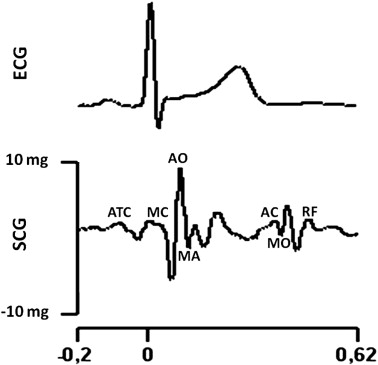
\includegraphics[width=0.6\textwidth]{Billeder/dirienzoetal2013.png}
   \caption{Et EKG sat over SCG. Taget fra Di Rienzo et al., 2013 \cite{di2013wearable}.} 
   \label{ecgscg}
\end{figure}

Følgende annotationer, som beskriver den mekaniske aktivitet i hjertet, er fremsat af Crow et al., 1994 \cite{crow1994relationship}\cite{paukkunen2014seismocardiography}:
\begin{itemize}
    \item AS, peak of atrial systole, her betegnet ATC for atrial contraction
    \item MC, mitral valve closure
    \item IM, isovolumic movement, her ikke-angivne dal mellem MC og AO, foreslået IVC for isovolumic contraction af Akhbardeh et al., 2009 \cite{akhbardeh2009comparative}
    \item AO, aortic valve opening
    \item IC, isotonic contraction, her angivet MA for den maximal acceleration, foreslået af Gurev et al., 2012 \cite{gurev2012mechanisms}
    \item RE, peak of rapid systolic ejection, her ikke-angivne bølge efter MA
    \item AC, aortic valve closure
    \item MO, mitral valve opening
    \item RF, peak of rapid diastolic filling
\end{itemize}

Disse annotationer bruges videre ud fra kendskab om hjertets virkemåde, herunder hjertets cyklus.
Hjertets cyklus opdeles i to perioder, den systoliske og diastoliske periode. Den systoliske periode indeholder PEP, IVCT og LVET. Den diastoliske periode indeholder IVRT. \cite{di2013wearable}

\textbf{PEP, pre-ejection period}, er defineret som tiden mellem Q-bølgen i EKG’et, og åbningen af aortaklappen. Denne indeholder bl.a. IVCT, og er tiden fra kontraktion af ventriklen sker, og frem til at udpumpning af blod kan forløbe grundet aortaklappens åbningen. Større PEP kan være en indikator for venstresidet hjertesvigt, som følge af lavere evne til sammentrækning. \cite{di2013wearable}

\textbf{IVCT, den isovolumetriske kontraktionstid}, er defineret som tiden mellem lukningen af mitralklappen, og åbningen af aortaklappen. Som navnet angiver, sker der ikke nogen volumetrisk ændring i denne periode. Der sker hverken en til- eller frastrømning fra venstre ventrikel. Da der sker en kontraktion, øges trykket imidlertid, hvilket hjælper med at føre blodet ud i aorta i den efterfølgende LVET periode. \cite{di2013wearable}

\textbf{LVET, left ventricular ejection time}, er defineret som tiden mellem åbningen og lukningen af aortaklappen. Denne periode beskriver derved udstrømningen af blod til aorta fra ventriklen. Som ved PEP, er denne også en indikator for venstresidet hjertesvigt, hvor lavere evne til sammentrækning fremkommer som en forlængelse af denne periode. \cite{di2013wearable}

\textbf{IVRT, den isovolumetriske reflektionstid}, er defineret som tiden mellem lukningen af aortaklappen og åbningen af mitralklappen. Som navnet angiver, sker der ikke nogen volumetrisk ændring i denne periode. Der sker hverken en til- eller frastrømning fra venstre ventrikel. Da der sker en afslapning af ventriklen, skabes et undertryk, hvilket hjælper med at føre blod ind i ventriklen ved den efterfølgende åbning af mitralklappen. \cite{di2013wearable}
 
De beskrevne perioder kan illustreres ved brug af et udvidet Wiggers diagram, hvor SCG’et er inkluderet, se figur \ref{wigdiagram}.

\begin{figure}[H]
\centering
  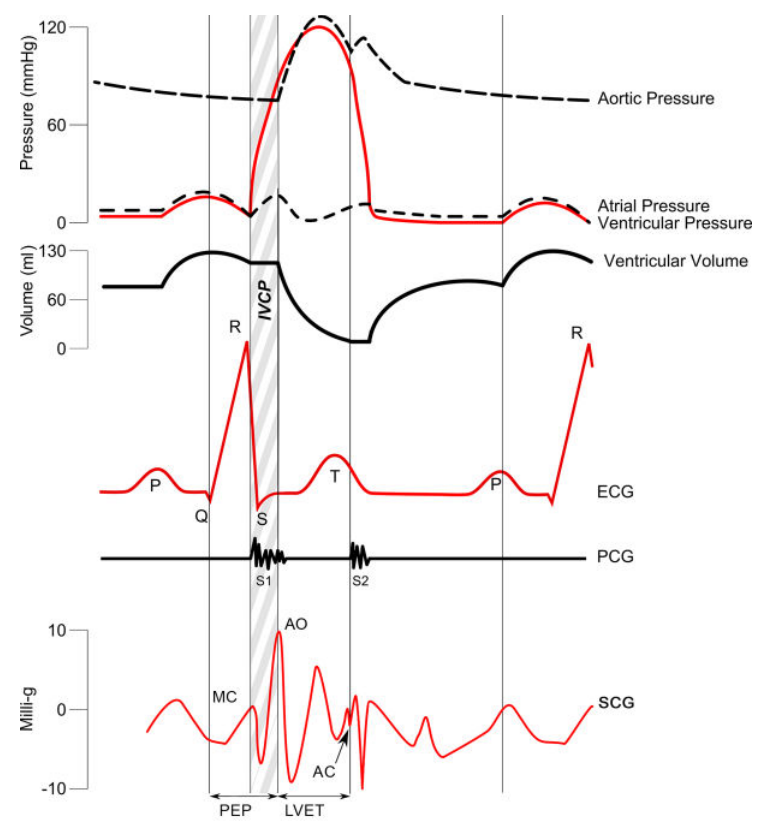
\includegraphics[width=0.7\textwidth]{Billeder/WiggersmedSCGZanetti.PNG}
   \caption{Et modificeret Wigger's diagram, hvor SCG er tilføjet. Tryk i ventrikel, atrie og aorta, samt volumen i ventriklen er vist. Yderligere er enkelte vigtige annotationer for SCG’et angivet. Taget fra Zanetti og Tavakolian, 2013 \cite{zanetti2013seismocardiography}.} 
   \label{wigdiagram}
\end{figure}

På figur \ref{wigdiagram} kan ses ændringerne i tryk og volumen, som følge af de mekaniske aktiviteter. Der ses en forøgelse i ventrikulært tryk, som følge af isovolumetrisk kontraktion, en forøgelse i aortisk tryk samt fald i ventrikulært volumen følgende isovolumetrisk kontraktion, samt stort fald i ventrikulært tryk som følge af isovolumetrisk relaksation. Isovolumetrisk relaksation er ikke illustreret, men dækkende fra starten til slutningen af anden hjertelyd på PCG’et, S2, og markerer slutningen af systolen og starten på diastolen \cite{zanetti2013seismocardiography}.


%[DER SKAL SÆTTES KILDER PÅ, OG SÅ SKAL AFSNITTET OVERORDNET REVURDERES IFT. GENTAGELSER, RENERE SPROG, DEFINITIONER (DANSK/ENGELSK NAVN) ETC.]\\
%Primære kilde ift. billede og beskrivelse: https://www-sciencedirect-com.zorac.aub.aau.dk/science/article/pii/S1566070213000805


\section{QRS kompleks signaler sammenlignet med SCG }


% \subsection{Hjertet}

\subsection{Elektrokardiogram}

\begin{figure}[H]
\centering
  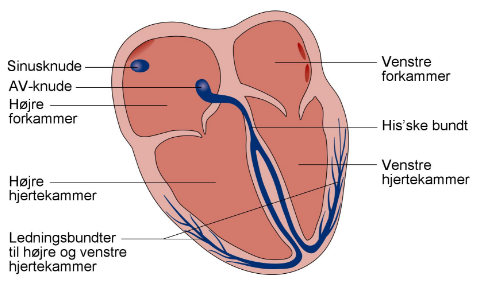
\includegraphics[width=0.6\textwidth]{Billeder/hjerte.png}
   \caption{Hjertets anatomi fra sundhed.dk} 
   \label{fig:hjerte}
\end{figure}

Hvert hjerteslag udløses af en lille specialiseret gruppe af celler, som kaldes sinusknuden og er hjertets naturlige pacemaker. Sinusknuden har evnen til at udløse elektriske signaler - også kaldet impulser - som er begyndelsen på et hjerteslag. 

Fra sinusknuden breder elektriske impulser sig igennem hjertet, som får hjertemuskelfibrene til at trække sig sammen. Efter at have aktiveret atrierne fra top til bund, fortsætter impulsen gennem AV-knuden. Denne er normalt kun et knudepunkt i det elektriske system mellem atrierne og ventriklerne. Impulsen forsinkes cirka et tiendedels sekund i AV-knuden, så atrierne får tid til at fylde ventriklerne med blod. 

Fra AV-knuden breder impulsen sig ned gennem His'ske bundt og ud i højre og venstre ventrikel. 

Rækkefølgen af det elektriske impuls vej under et hjerteslag opsummeret:
\begin{itemize}
    \item Sinusknude (højre atrium)
    \item Sammentrækning af atrier
    \item AV-knude (mellem atrier og ventrikler)
    \item Stimulering af His'ske bundt og Purkinje fibre
    \item Sammentrækning af ventrikler
\end{itemize}

\begin{figure}[H]
\centering
  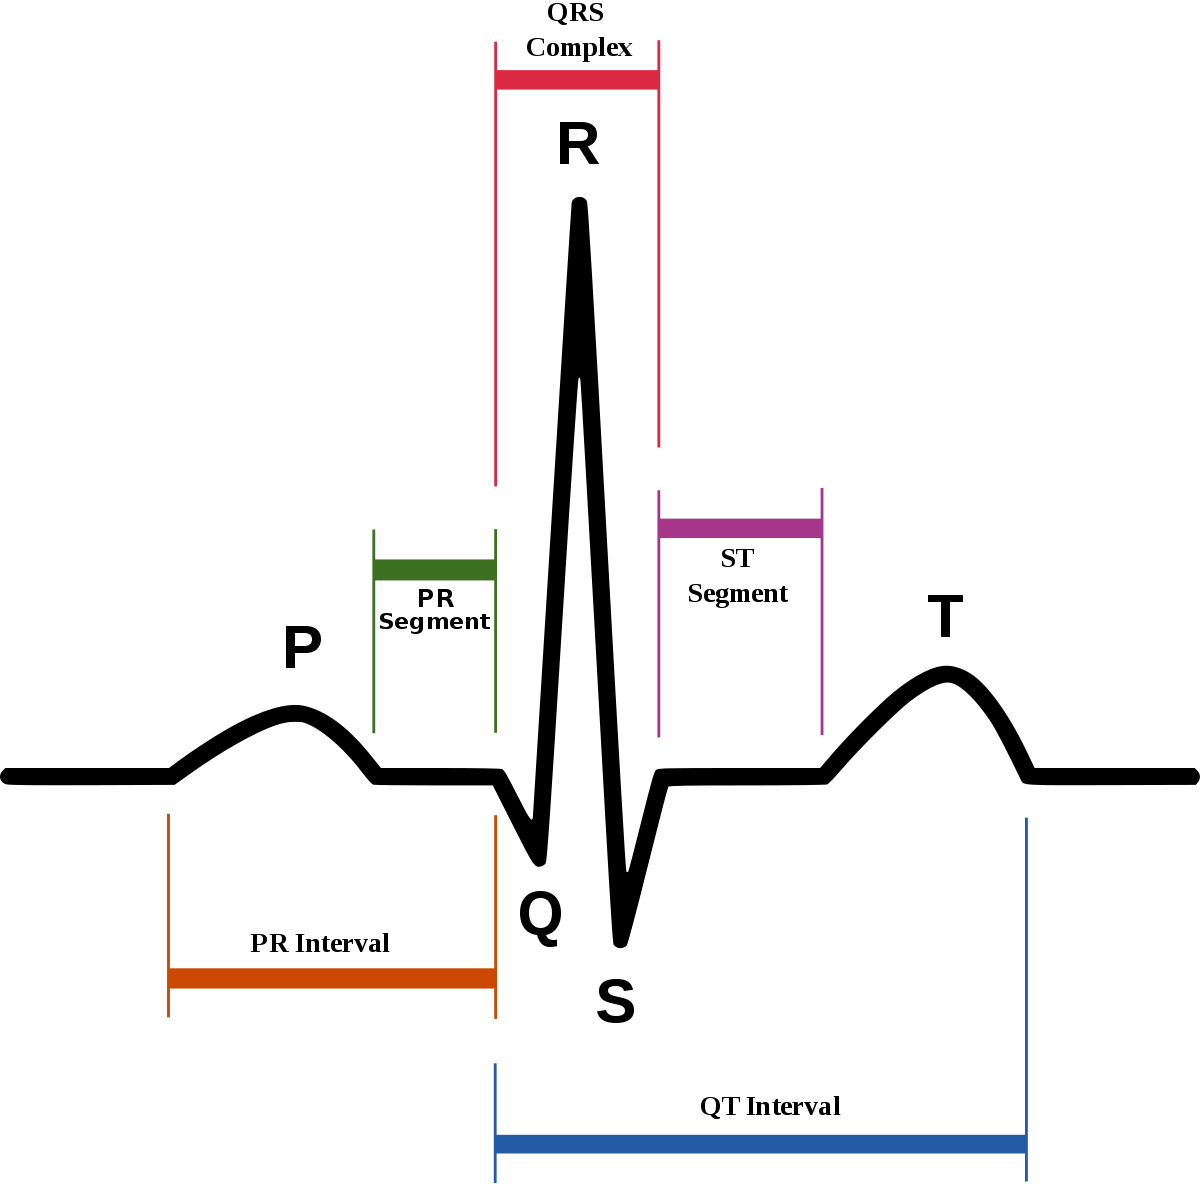
\includegraphics[width=0.6\textwidth]{Billeder/pqrst.png}
   \caption{EKG signal} 
   \label{fig:pqrst}
\end{figure}

\textbf{P bølge} repræsenterer depolarisering af atrierne. Impulser spredes fra sinusknude mod AV-knude og fra højre til venstre atrium. Kontraktion af atrierne forekommer 25 msek efter starten af p bølgen.

\textbf{PR interval} måles fra starten af p bølgen og til starten af QRS komplekset. Dette interval repræsenter den tid det tager for den elektriske impuls at rejse fra sinusknude til AV-knude.

\textbf{PR segment} er den flade linje mellem slutningen af p-bølgen og starten af QRS komplekset. Denne reflekterer den tids forsinkelse af AV-knude som forekommer således at ventriklerne kan fyldes.  

\textbf{QRS komplekset} repræsenterer den hurtige depolarisering af ventriklerne. Det elektriske signal er meget stærk, da ventriklernes muskler er meget mere massiv ift atrierne. 

\textbf{ST segment} forbinder QRS kompleks med t bølge. Repræsenter den tid det tager for ventriklerne at depolarisere.

\textbf{T bølge} repræsenter repolarisering af ventriklerne. Repolarisering af artierne ses ikke i EKG'et, da det finder sted mens ventriklerne depolariserer og QRS komplekset forekommer. 

\subsection{Pre- og afterload}

\textbf{Slagvolumen} er den mængde blod, som pumpes ud fra hjertet under hvert pulsslag, hos mennesket ca. 80 ml.

\textbf{Minutvolumen/cardiac output} er den mængde blod, hjertet pumper ud pr. minut; udregnes som produktet af hjertets slagvolumen og slagfrekvensen, dvs. pulsen. Hjertets minutvolumen er hos voksne personer i hvile ca. 5 l/min. 

Preload og afterload er to afgørende faktorer for, hvor meget blod hjertet pumper i et minut (minutvolumen).

\textbf{Preload} defineres som den mængde af blod som kommer ind i ventriklerne lige før hjertet kontraherer (systole). Mere blod giver mere udstrækning af ventriklerne, hvilket giver en øget preload. Jo større preload, jo kraftigere kontraktion og jo større slagvolumen. 

\textbf{Afterload} defineres som den mængde af modstand/tryk som ventriklen skal overkomme for at blodet kan bevæge over i aorta under systole. Hvis afterload øges (eksempelvis pga. hypertension) så vil den isovolumetriske kontraktionsfase forlænges fordi ventriklerne har brug for at generere et højere tryk og slagvolumen nedsættes. 


% \chapter{Metode}

Følgende er fra \cite{Arlow2002}
\section{Unified process}
Unified process (UP) er en softwareudviklingsmetode. 

\subsection{Overordnede principer}

\textbf{Iterativ} metode benyttes ved UP og beskriver en situation hvor projektet brydes ned til mindre subprojekter (iterationer) som gør fremgangsmåden lettere at håndtere og udføre succesfuldt. Hver iteration giver systemet funktionalitet og når iterationen giver en udvidelse af det færdige system betegnes denne inkrementel. På denne måde bygges softwaren trinvist op og som i sidste ende fører til et fuldt funktionelt system. Ved at bryde projektet ned i en serie af iterationer tillader det en fleksibel tilgang til projekt planlægningen sammenlignet med den gamle vandfaldsmodel som er udformet i mere strikse sekvenser.

\textbf{Use case} ligger fundamentet for udviklingen. Formålet med iteration er som regel at udvikle en eller flere use cases.

\textbf{Arkitektur-centreret} beskriver hvordan systemet brydes ned i komponenter, og hvordan disse interagerer og implementeres. 

\textbf{Risiko-drevet} fokuserer på at identificere risici tidligt, hvorved det bliver muligt at identificere hvilke use-cases der vil være optimalt at koncentrere sig om i starten.

\subsection{Iterationer}
Hver iteration indeholder alle elementer i en almindelig software udviklings projekt; planlægning, analyse og design, konstruktion, integration og test, en intern eller ekstern udgivelse. For hver iteration findes der fem kerneelementer:
\begin{itemize}
    \item Krav: Hvad skal systemet kunne?
    \item Analyse: Raffinere og strukturer krav
    \item Design: Realisere krav i et system arkitektur
    \item Implementering: Bygge softwaren
    \item Test: Verificere at implementering virker som ønsket 
\end{itemize}

\subsection{Struktur}
UP er overordnet delt ind i fire faser. Hver fase kan have en eller flere iterationer, og for hver iteration udføres de fem kerneelementer. Mængden af arbejde der lægges i de fem kerneelementer ændres i de forskellige faser i takt med at projektet skrider frem, se figur \ref{fig:UP}.
\begin{itemize}
    \item \textbf{Forberedelse}: De grundlæggende visioner for systemet og et overblik over kravene fastslås. Desuden identificeres risici og formål defineres. 
    \item \textbf{Etablering}: Der fastlægges en grundlæggende arkitektur. Systembeskrivelse og kravspecifikationer defineres. Fokus i etableringsfasen er på krav, analyse og design elementerne. I slutningen af denne fase bliver implementering et vigtigt element, når den grundlæggende arkitektur er produceret.  
    \item \textbf{Konstruktion}: Systemets funktioner udvikles og testes. Målet er at færdiggøre alle krav, analyse og design og udvikle det endelig system. I denne fase vægtes implementeringselementet. 
    \item \textbf{Overdragelse}: Overgangen hvor systemet leveres til slutbrugeren. 
\end{itemize}

\begin{figure}[H]
\centering
  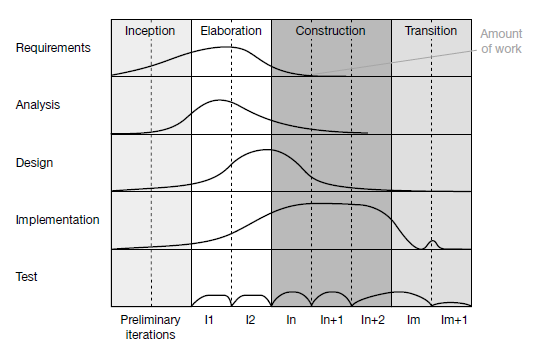
\includegraphics[width=0.8\textwidth]{Billeder/UP.png}
   \caption{Kolonerne i figuren repræsenterer faserne mens rækkerne repræsenterer de fem kerneelementer. Figuren illustrerer hvordan arbejdsfordeling af de fem kerneelementer varierer afhængig af hvilken fase man befinder sig i. \cite{Arlow2002}} 
   \label{fig:UP}
\end{figure}

%Kunne godt tænke mig at komme tænke mig at vide mere om hvad de 5 kerne elementer indebærer 

\section{Objekt orienteret programmering}

%Der findes tre grundprincipper i objektorienteret programmering; indkapsling, nedarving og polymorfi. Et objekt indkapsler nogle data og noget funktionalitet (adfærd). Nedarving. Et objekt kan arve data og funktionalitet fra et andet objekt og udvide med med ekstra data og funktionalitet. Polymorfi. To klasser han kave samme grænseflade defineret via nedarving, men udføre dem forskelligt. Java er et eksempel på et almindeligt objektorienteret sprog og systemet er opbygget af indbyrdes sammemhængende objekter. Der er altid et overordnet objekt som instantierer et andet objekt, dvs. laer sin egen kopi af et andet objekt. 
Objektorienteret programmering er et paradigme indenfor softwareudvikling. Den overordnede filosofi er at definere et softwaresystem bestående af en samling af objekter som interagerer med hinanden.  Programmeringskoden opdeles i klasser, som hver har sit ansvarsområde i programmet. Et objekt er en instans af en klasse og en klasse kan således genbruges adskillige gange til at skabe objekterne. Klassen er en skabelon som definerer objektets adfærd og består overordnet af to delelementer; attributter og metoder. Attributter definerer objektets egenskaber mens metoder definerer de mulige funktioner som objektet kan udføre. \cite{Dathan}  

\section{Unified Modeling Language (UML)}

UML er en standard for diagrammer, som beskriver objektorienteret programmering.

\textbf{Krav} Før analyse og design påbegyndes, er der behov for at kravspecifikationerne defineres. Krav danner basis for systemet og fortæller hvad synes skal kunne gøre. Der findes to typer af krav; de funktionelle kravspecifikationer som udledes ud fa use cases og ikke funktionelle krav som omhandler begrænsinger af systemet. 

\textbf{Use case} Først defineres aktører som direkte interagerer med systemet og findes eksternt for systemet. Derefter opstilles use cases som er noget en aktør ønsker systemet skal kunne gøre. 

\textbf{Analyse} Skabe modeller som fortæller om systemets ønskede adfærd. Producer analyse modeller som fokuserer på hvad systemet skal kunne gøre mens hvordan det skal gøres overlades til design. 

Use case realizations: samarbejdet mellem objekter som viser hvordan integaktion mellem objekter kan realiserer en adfærd udtrykt i use cases. 

Find klasser til objekterne. Klasser består af et sæt af attributer. 

Problem domænet: domæne hvori brugen for et software system opstår. 

\begin{itemize}
    \item Krav: Brugere samt deres behov, hvorudfra der opstilles krav til systemet. Der udarbejdes use cases. Funktionelle og ikke funktionelle krav. 
    \item Analyse: aktivitivitetsdiagrammer for hver use case med forbindelseselementer. Analyseklasse; hvad skal den kunne men ikke hvordan. Analysediagram: hver klasse samt dens egenskab og relation til hinanden. 
    \item Design: Specificer hvordan funktionaliteten kan implementeres. Sekvensdiagrammer; hvordan og hvornår i koden forskellige use cases skal benyttes for at opnå den ønskede funktionalitet. 
    \item Implementering: kodning af de designede modeller. Java. 
    \item Test: test softwarens funktionalitet; white box og black box test. 
\end{itemize}

Brugergrænseflade designprincipper > GUI
% \section{SCRUM}
\textit{}

SCRUM er en organisatorisk tilgang til udførelsen af et produkt, primært softwareudvikling. Ved brug af SCRUM fremsættes en overordnet liste, en backlog, af planlagt indhold og egenskaber, disse prioriteres, og det videre arbejde planlægges i mindre segmenter.
Forud for en forklaring af de forskellige faser i SCRUM, bør de forskellige roller indeholdt i SCRUM forklares. Der findes tre primære roller tilhørende SCRUM: Ejeren, udviklerne, og SCRUM masteren.


\textbf{Ejeren} fastsætter produktets omfang, backloggen, i form af indhold og egenskaber, og ejeren står med ansvaret for dette. Disse skal også rangeres, og mens dette kan overlades til udviklerne, skal disse stadig forhøre sig hos ejeren for eventuelle ændringer til en prioriteret liste.\\
\textbf{Udviklerne} står for udarbejdelse af produktet. Disse holdes ansvarlige for at bidrage med fremskredne dele af produktet, ift. Sprint deadlines. Set ift. SCRUM, inddeles udviklerne ikke i mindre hold eller roller. Alle er lige ansvarlige for at et potentielt udgivelsesparat produkt er færdigt ved Sprint deadline.\\
\textbf{SCRUM masteren} er ansvarlig for optimal brug af SCRUM hos både ejeren og udviklerne. Denne hjælper ejeren med organisation af produktets backlog, således opgaverne med højest prioritet, hvad enten det er praktikalitet eller andet, udføres først. Yderligere hjælper SCRUM masteren udviklerne med at få en god forståelse for SCRUM, således opgaverne der udføres bliver gjort på bedste vis.\\


SCRUM i sig selv inddeles i forskellige dele og faser. Forud samt under udvikling af et produkt, findes en backlog for produktet. I backloggen findes alle dele af produktet. Backloggen fastsættes før arbejde på produktet påbegyndes, og denne ændres løbende som krav for produktet ændres eller udføres. Ejeren står for udarbejdelse og opdatering af backloggen, og dette gøres ofte i samarbejde med udviklerne. Efterfølgende for udarbejdelse af en produkt backlog holdes et Sprint planlægningsmøde. På baggrund af produkt backloggen samt planlægningen for den opkommende Sprint, udarbejdes en Sprint backlog, hvor arbejde som anses af høj prioritet for et udgivelsesparat produkt uddelegeres til udviklerne. Denne skal være detaljeret, således det er muligt på det daglige SCRUM møde at beskrive ændringer for planlagt fremskridt af Sprint. En Sprint er omtrent 2-4 uger i længde, og det arbejde som planlægges udført ændres ikke undervejs. Der arbejdes ikke på baggrund af hvad der er planlagt udført i Sprint backloggen, men udelukkende på baggrund af den afsatte mængde tid. Efterfølgende for en Sprint udarbejdes en opdatering for Sprint backloggen, og en ny Sprint påbegyndes. Undervejs i Sprint afholdes daglige møder, hvor det kommende døgn diskuteres for udvikling af produktet. Samtidig bruges det daglige møde som en synkronisering for udviklerne.


Overordnet kilde: Scrum.org → Skal have skrevet lidt flere på, som scrumguide.org og scrumalliance.org osv.

%
\section{Kravspecifikationer}
På baggrund af systembeskrivelsen opstilles en række kravspecifikationer for en app der optager SCG til telemonitorering af hjertesvigtpatienter. Disse krav er inddelt i funktionnel og ikke-funktionelle. De funktionelle krav relaterer sig til selve app'ens funktionalitet, mens de non-funktionelle har betydning for brugervenligheden. For hvert krav er desuden specificeret, hvorfor kravet er medtaget.

%Der opstilles på baggrund af systembeskrivelsen kravspecifikationer for app’en. Disse krav opstilles i funktionelle og non-funktionelle, hvor de funktionelle krav er relevante for app’ens funktionalitet, og de non-funktionelle er relevante for brugervenligheden.

\textbf{Funktionelle krav}
\begin{itemize}
    \item Brugeren skal kunne oprettes i databasen. \textit{Dette sikrer at brugernes data kan lagres, så de kan tilgås af en læge.}
    \item Brugeren skal være tilknyttet personligt ID og password. \textit{Dette er nødvendigt for at sikre individuel lagring af brugerdata, så data for hver bruger kan monitoreres og analyseres individuelt.}
    \item Systemet skal kunne tilgå smartphone'ens accelerometer. \textit{Det er nødvendigt for systemet at tilgå smartphone'ens accelerometer, således seismokardiografisk måling kan udføres og lagres.}
    \item Systemet skal kunne optage ændringer i acceleration. \textit{Da seismokardiografi baserer sig på ændringer i acceleration, er dette nødvendigt for udførelse af måling.}
    \item Systemet skal kunne måle tid i minutter og sekunder. \textit{Dette er nødvendigt for at angive en tidsakse for seismokardiografi-målingen.}
    \item Brugeren skal kunne tilgå en brugsanvisning for udførsel af målinger. \textit{Dette er nødvendigt for at hjælpe brugeren med at udføre korrekt måling.}
    \item Brugeren skal kunne indtaste relevante informationer i systemet
Dette er nødvendigt for korrekt oprettelse af personen hos lægen. Oplysninger omfatter CPR, medicin, symptomer m.m.
    \item Brugeren skal kunne starte målinger. \textit{Dette er nødvendigt for at få målinger.}
    \item Systemet skal kunne afslutte målinger efter specifik tidsperiode. \textit{Dette er nødvendigt for at få målinger af samme længde, uden at brugere selv skal stoppe målingen.}
    \item Brugeren skal kunne indtaste oplysninger efter endt måling
Dette er nødvendigt for at angive brugerens aktivitet forud for måling, såsom motion.
    \item Systemet skal kunne starte ny måling over gamle uden at sende den gamle måling til databasen. \textit{Dette er nødvendigt hvis der opstår komplikationer undervejs. Dette kunne eksempelvis være større bevægelse af brystkassen, der ville give en dårlig måling.}
    \item Brugeren skal kunne stoppe målingen undervejs. \textit{Dette er nødvendigt for at brugeren kan stoppe målingen hvis komplikationer opstår undervejs.}
    \item Systemet skal kunne påminde brugeren om at foretage nye målinger. \textit{Dette er nødvendigt for at sikre, at brugeren foretager målinger ofte nok.}
    \item Brugeren skal kunne ændre password. \textit{Dette er nødvendigt for at give brugeren mulighed for at ændre password.}
    \item Brugeren skal kunne logge ud af app’en. \textit{Dette beskytter mod uvedkommende tilgang til brugerens data.}
\end{itemize}

\textbf{Non-funktionelle krav}:
\begin{itemize}
    \item Systemet skal være brugervenligt
Dette er nødvendigt for at brugeren lettere kan tilgå og udføre målinger.
    \item Systemet skal kunne visualiseres på en smartphone
\end{itemize}


%% Syntese %%

%%%% Kilder %%%%

\begingroup
	\raggedright
	\bibliography{bibtex/litteratur}							% Litteraturlisten inkluderes
\endgroup


%%%% Fixme-listen %%%%

%\newpage														% Ny side til Fixme-listen													% Fixme-listen - fjernes til sidst i projektet med "%"


%%%% Appendiks %%%%

\appendix														% Appendiks/bilag start - giver chapter bogstaver i stedet for tal
\clearforchapter												% Sikrer at pagestylen aktiveres paa den rigtige side
\phantomsection													% Kunstigt afsnit, som hyperlinks kan 'holde fast i'
\pdfbookmark[0]{Appendiks}{appendiks}							% Tildeler en klikbar bookmark til den endelige PDF

%% Indstillinger for appendiks (deaktiveret med "%") %%

%\pagestyle{empty}												% Sidehoved/-fod for standardsider aendres til tom for appendiks
%\aliaspagestyle{chapter}{empty}								% Sidehoved/-fod for kapitelsider aendres til tom for appendiks
%\settocdepth{chapter}											% Kun kapitel-niveau vises i ToC
%\addtocontents{toc}{\protect\cftpagenumbersoff{chapter}}		% Sidetal for kapitler fjernes i ToC

%% Filer til appendiks indsættes her %%



%%%% Bilag %%%%

%\phantomsection												% Kunstigt afsnit, som hyperlinks kan 'holde fast i'
%\addcontentsline{toc}{chapter}{Bilag A \ Navn} 				% Manuelle indgange i indholdsfortegnelsen (naar \includepdf bruges)

%\includepdf[pages={x-y}]{filnavn}								% Inkluder eksterne bilag med \includepdf[pages={x-y}]{filnavn}


\end{document}													% Slutter dokumentet - obligatorisk


